%*******************************************************************************
%****************************** Second Chapter *********************************
%*******************************************************************************

\chapter{IoT và Các kiến thức cơ bản về IoT}

\ifpdf
    \graphicspath{{Chapter2/Figs/Raster/}{Chapter2/Figs/PDF/}{Chapter2/Figs/}{Chapter2/Figs/web/}}
\else
    \graphicspath{{Chapter2/Figs/Vector/}{Chapter2/Figs/}}
\fi


%\section[Short title]{Reasonably long section title}
\section{Giới thiệu về Internet of Things và các ứng dụng giám sát}
\subsection{Internet of Things (IoT)}
Với sự phát triển nhanh chóng của công nghê máy tính hiện nay, những công nghệ cao đã đang và ngày càng được ứng dụng trong nhiều lĩnh vực của cuộc sống con người. IoT là mạng lưới của các đối tượng vật lý, các thiết bị, các phương tiện và các đối tượng này được nhúng với các thiết bị điện tử, cảm biến, phần mềm điều khiển, và nó có khả năng trao đổi dữ liệu và thao tác với nhau. IoT cho phép các đối tượng được lắng nghe và điều khiển từ xa trên cơ sở hạ tầng mạng hiện có, các hệ thống máy tính có thể thu thập dữ liệu và điều khiển các thiết bị đối tượng một cách hiệu quả, chính xác và lợi ích kinh tế nhất có thể. 
\begin{figure}[htbp!] 
\centering    
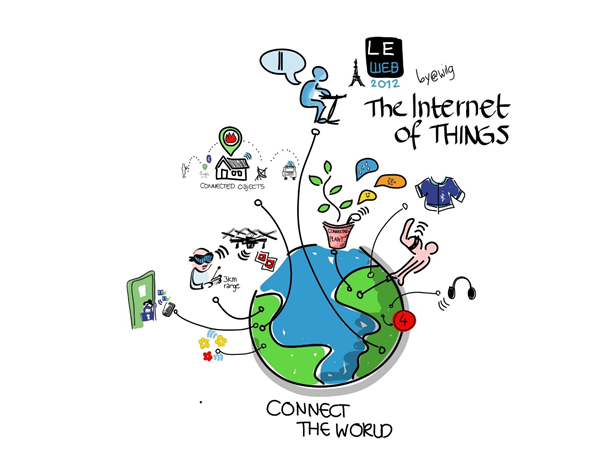
\includegraphics[width=1.0\textwidth]{pic4}
\caption[Hình ảnh mô tả Internet of Things ]{Hình ảnh mô tả Internet of Things }
\label{fig:pic4}
\end{figure}


\subsection*{Khả năng định danh độc nhất }
Điểm quan trọng của IoT đó là các đối tượng phải có thể được nhận biết và định dạng. Nếu mọi đội tượng, kể cả con người, được "đánh dấu" để phân biệt bản thân đối tượng đó với những thứ xung quanh thì chúng ta có thể hoàn toàn quản lí được nó thông qua máy tính. Việc đánh dấu có thể được thực hiện thông qua nhiều công nghệ, chẳng hạn như RFID, NFC, mã vạch, mã QR, watermark kĩ thuật số... Việc kết nối thì có thể thực hiện qua Wi-Fi, mạng viễn thông băng rộng (3G, 4G), Bluetooth, ZigBee, hồng ngoại...
Ngoài những kĩ thuật nói trên, nếu nhìn từ thế giới web, chúng ta có thể sử dụng các địa chỉ độc nhất để xác định từng vật, chẳng hạn như địa chỉ IP. Mỗi thiết bị sẽ có một IP riêng biệt không nhầm lẫn. Sự xuất hiện của IPv6 với không gian địa chỉ cực kì rộng lớn sẽ giúp mọi thứ có thể dễ dàng kết nối vào Internet cũng như kết nối với nhau.

\subsection*{Xu hướng và tính chất của The Internet of Things }
\textbf{Thông minh:} Sự thông minh và tự động trong điều khiển thực chất không phải là một phần trong ý tưởng về IoT. Các máy móc có thể dễ dàng nhận biết và phản hồi lại môi trường xung quanh (ambient intelligence), chúng cũng có thể tự điều khiển bản thân (autonomous control) mà không cần đến kết nối mạng. Tuy nhiên, trong thời gian gần đây người ta bắt đầu nghiên cứu kết hợp hai khái niệm IoT và autonomous control lại với nhau. Tương lai của IoT có thể là một mạng lưới các thực thể thông minh có khả năng tự tổ chức và hoạt động riêng lẻ tùy theo tình huống, môi trường, đồng thời chúng cũng có thể liên lạc với nhau để trao đổi thông tin, dữ liệu.

Việc tích hợp trí thông minh vào IoT còn có thể giúp các thiết bị, máy móc, phần mềm thu thập và phân tích các dấu vết điện tử của con người khi chúng ta tương tác với những thứ thông minh, từ đó phát hiện ra các tri thức mới liên quan tới cuộc sống, môi trường, các mối tương tác xã hội cũng như hành vi con người.

\textbf{Kiến trúc dựa trên sự kiện:} Các thực thể, máy móc trong IoT sẽ phản hồi dựa theo các sự kiện diễn ra trong lúc chúng hoạt động theo thời gian thực. Một số nhà nghiên cứu từng nói rằng một mạng lưới các sensor chính là một thành phần đơn giản của IoT.

\textbf{Là một hệ thống phức tạp:}Trong một thế giới mở, IoT sẽ mang tính chất phức tạp bởi nó bao gồm một lượng lớn các đường liên kết giữa những thiết bị, máy móc, dịch vụ với nhau, ngoài ra còn bởi khả năng thêm vào các nhân tốc mới.

\textbf{Kích thước: } Một mạng lưới IoT có thể chứa đến 50 đến 100 nghìn tỉ đối tượng được kết nối và mạng lưới này có thể theo dõi sự di chuyển của từng đối tượng. Một con người sống trong thành thị có thể bị bao bọc xung quanh bởi 1000 đến 5000 đối tượng có khả năng theo dõi.

\textbf{Vấn đề không gian, thời gian: }Trong IoT, vị trí địa lý chính xác của một vật nào đó là rất quan trọng. Hiện nay, Internet chủ yếu được sử dụng để quản lí thông tin được xử lý bởi con người. Do đó những thông tin như địa điểm, thời gian, không gian của đối tượng không mấy quan trọng bởi người xử lí thông tin có thể quyết định các thông tin này có cần thiết hay không, và nếu cần thì họ có thể bổ sung thêm. Trong khi đó, IoT về lý thuyết sẽ thu thập rất nhiều dữ liệu, trong đó có thể có dữ liệu thừa về địa điểm, và việc xử lí dữ liệu đó được xem như không hiệu quả. Ngoài ra, việc xử lí một khối lượng lớn dữ liệu trong thời gian ngắn đủ để đáp ứng cho hoạt động của các đối tượng cũng là một thác thức hiện nay.

\newpage

\subsection*{Mô hình theo xu hướng IoT thực tế}
Mô hình (Hình ~\ref{fig:pic5}): Các thiết bị sẽ có thể kết nối với nhau bằng TCP/UDP và có thể kết nối trực tiếp đến máy chủ mà không cần thông qua thiết bị khác.

\begin{figure}[htbp!] 
\centering    
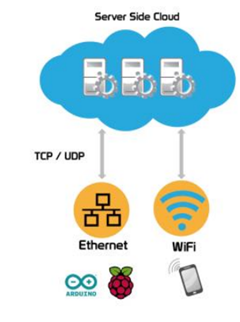
\includegraphics[width=0.5\textwidth]{pic5}
\caption[Mô hình IoT không có Gateway ]{Mô hình IoT không có Gateway}
\label{fig:pic5}
\end{figure}

Mô hình (Hình ~\ref{fig:pic6}): Các thiết bị sẽ được hỗ trợ nhiều chuẩn giao tiếp khác nhau (BLE, ZWave,…) nên cần cầu nối là Gateway để kết nối đến máy chủ. 
	
	

\begin{figure}[htbp!] 
\centering    
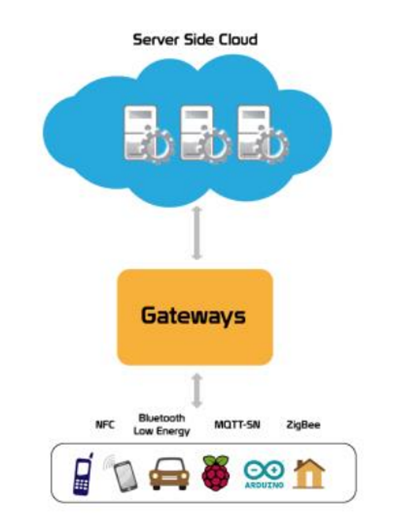
\includegraphics[width=0.5\textwidth]{pic6}
\caption[Mô hình IoT có Gateway]{Mô hình IoT có Gateway}
\label{fig:pic6}
\end{figure}


Sơ đồ lớp Chung của cả hai mô hình trên:


\begin{figure}[htbp!] 
\centering    
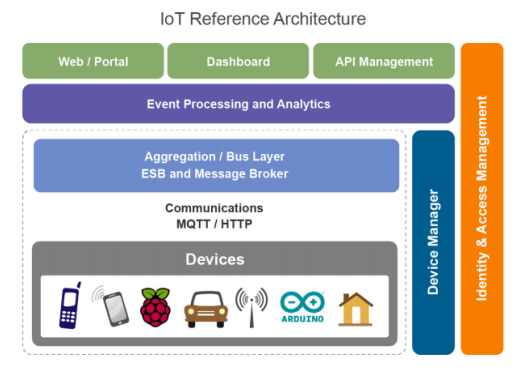
\includegraphics[width=1\textwidth]{pic7}
\caption[Kiến trúc mô hình IoT tham khảo]{Kiến trúc mô hình IoT tham khảo}
\label{fig:pic7}
\end{figure}



\begin{itemize}
\item[•]Lớp Device \\
Lớp dưới cùng của kiến trúc là lớp thiết bị. Thiết bị có thể được các loại khác nhau, nhưng để có thể được xem là thiết bị IOT, nó phải có một số thông tin liên lạc hoặc gián tiếp hoặc trực tiếp với Internet.\\
Mỗi thiết bị thường cần một ID. ID có thể là: Bluetooth identifier, Wi-Fi MAC Address…
\item[•]Lớp Communications \\
Các lớp truyền thông hỗ trợ các kết nối của các thiết bị tới máy chủ. Có nhiều giao thức để giao tiếp giữa các thiết bị và máy chủ. Nổi bật nhất là HTTP hoặc MQTT.\\
HTTP rất thông dụng. Bởi vì nó là một giao thức dựa trên văn bản đơn giản, nhiều thiết bị nhỏ như bộ điều khiển 8-bit có thể hỗ trợ một phần các giao thức - ví dụ đủ dữ liệu để POST hoặc GET một nguồn tài nguyên. Các thiết bị lớn hơn 32-bit có thể sử dụng đầy đủ các thư viện HTTP client đúng cách để hiện thực toàn bộ giao thức.\\
MQTT được phát minh vào năm 1999 để giải quyết các vấn đề trong hệ thống nhúng và SCADA. Nó đã được thông qua một số lần lặp lại và phiên bản hiện tại (3.1.1) đang trải qua những tiêu chuẩn hoá trong OASIS MQTT kỹ thuật Committee8. MQTT là một hệ thống tin nhắn publish-subscribe dựa trên một mô hình broker. Các giao thức có một chi phí rất nhỏ (ít nhất là 2 byte cho mỗi tin nhắn). MQTT được thiết kế để vận hành qua TCP.

\item[•]Lớp Aggregation/Bus \\
Một lớp quan trọng của kiến trúc là lớp mà tập hợp và là cầu nối, có khả năng tổng hợp và kết hợp các thông tin liên lạc từ các thiết bị khác nhau và đưa thông tin liên lạc đến một thiết bị cụ thể (có thể thông qua một gateway).
\item[•]Lớp Event Processing and Analytic: \\
Lớp này có các sự kiện từ lớp Bus và cung cấp khả năng xử lý và hành động theo những sự kiện này. Yêu cầu phải lưu trữ các dữ liệu vào một cơ sở dữ liệu nên buộc phải có một ứng dụng ở máy chủ.
\item[•]Lớp External Communications (Top) \\
Lớp này cung cấp một cách cho các thiết bị để chúng giao tiếp ra bên ngoài hệ thống một cách có định hướng và thân thiện với người dùng (Web, Dashboard, API Management)
\end{itemize}

% Please add the following required packages to your document preamble:

\begin{table}[]
\centering
\caption{My caption}
\label{my-label}
\begin{tabular}{|l|l|l|}
\hline
\textbf{MÔ HÌNH} & \textbf{ƯU ĐIỂM} & \textbf{NHƯỢC ĐIỂM} \\ \hline
\textbf{Mô hình cũ} & Đơn giản hiện thực & \begin{tabular}[c]{@{}l@{}}Gateway cồng kềnh vì phải có \\ bộ phận thu/phát hồng ngoại \\ và các mạch để giao tiếp RF.\end{tabular} \\ \hline
\textbf{Mô hình 1} & \begin{tabular}[c]{@{}l@{}}Không cần thông qua \\ gateway, mọi thông tin \\ thiết bị đều được lưu \\ trên máy chủ.\end{tabular} & \begin{tabular}[c]{@{}l@{}}Hạn chế về phương thức giao\\ tiếp vì chỉ sử dụng TCP/UDP \\ để giao tiếp. Không thể điều khiển\\  thiết bị khi không truy cập được \\ máy chủ.\end{tabular} \\ \hline
\textbf{Mô hình 2} & \begin{tabular}[c]{@{}l@{}}Quản lý thiết bị thông qua\\ gateway làm trung gian, nên\\ các thiết bị có thể tương tác\\ với nhau dễ dàng mà không \\ cần đến máy chủ.\end{tabular} & \begin{tabular}[c]{@{}l@{}}Chi phí cao hơn, hệ thống \\ phức tạp hơn. Độ bảo mật \\ cũng cần được quan tâm hơn.\end{tabular} \\ \hline
\end{tabular}
\end{table}



	
\subsection{Các hệ thống giám sát được phát triển dựa trên IoT}
Khi kết nối một chuỗi khổng lồ các cảm biến (sensor) thu thập dữ liệu, thiết bị và máy móc với nhau, điều quan trọng cần nhận ra là thông tin sẽ được chuyển đổi thành hành động với một tốc độ mà chúng ta chưa từng thấy trước kia. Chúng ta đang tiến đến gần, nếu không phải là đã chạm được vào một thế giới của những khoảng thời gian phản ứng cực nhỏ, phản hồi tức thì với mọi điều kiện biến đổi, và mức độ điều khiển chưa từng có trong việc quản lý tài nguyên và tài sản.
Điểm mấu chốt ở đây là đừng nghĩ hẹp. Internet of Things (IoT) không đơn thuần là mang đến sự tiết kiệm trong các mô hình công nghiệp hiện tại. Nó đảo lộn hoàn toàn những mô hình cũ, tạo ra những sản phẩm và dịch vụ mới. Không có một lĩnh vực nào mà trong đó IoT tạo ra ảnh hưởng đặc biệt lớn nhất; bởi IoT sẽ thay đổi hoàn toàn mọi lĩnh vực một cách không thể tưởng tượng được, bao gồm nông nghiệp, năng lượng, an ninh, quản lý thảm họa, y tế, và đó chỉ là một vài lĩnh vực được nhắc đến.

\subsection*{Ứng dụng trong xây dụng }
\begin{figure}[htbp!] 
\centering    
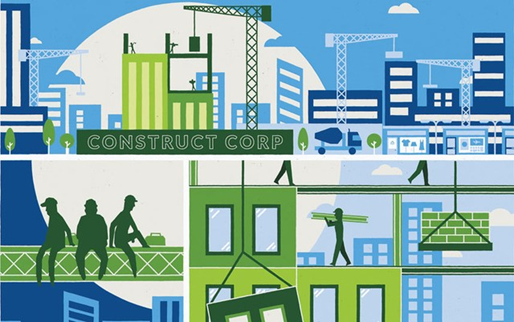
\includegraphics[width=1\textwidth]{pic8}
\caption[Ứng dụng IoT trong xây dựng ]{Ứng dụng IoT trong xây dựng }
\label{fig:pic8}
\end{figure}

Ví dụ: Các công ty xây dựng đã bắt đầu trang bị các silo (hầm chứa đồ) và xe tải có các cảm biến theo dõi mức hàng tồn kho, như là lượng bê tông, và biến đổi nó thông qua platform trên nền điện toán đám mây để gia tăng tốc độ phân phối và đảm bảo một dòng lưu thông vật liệu ổn định. Các ông lớn trong ngành công nghiệp dầu mỏ đã bắt đầu thực thi các công nghệ mobile, cảm biến tới máy móc để dự phòng từ trước cho các tai nạn thông qua các phân tích nhanh chóng và hành động tức thời. Khi các cảm biến phát hiện ra một sự cố như rò rỉ hoặc thất thoát đường ống, công nghệ IoT cho phép các công nhân lập tức xác định vị trí của chúng.

\subsection*{Ứng dụng trong năng lượng }

\begin{figure}[htbp!] 
\centering    
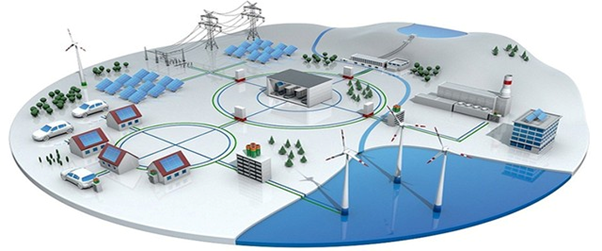
\includegraphics[width=1\textwidth]{pic9}
\caption[Ứng dụng IoT trong năng lượng]{Ứng dụng IoT trongnăng lượng}
\label{fig:pic9}
\end{figure}
Một ví dụ khác của công nghệ IoT mới ứng dụng trong công nghiệp dầu mỏ, đó là giếng thông minh. Đây là một dạng giếng cài đặt các thiết bị điều khiển dòng chảy và cảm biến lỗ khoan, để có thể giám sát và điều khiển từ trên bề mặt mà không đe dọa an toàn của công nhân. Giếng thông minh có trang bị công nghệ địa chấn 4D, cho phép theo dõi sự rò rỉ khí ga, dòng chảy nước, thay đổi áp lực, và bất cứ thay đổi nào khác gây ra bởi những biến động địa chấn, giúp cho việc dự đoán và điều khiển các tác động địa chấn có thể gây ra những hỏng hóc nghiêm trọng.
Nhưng như thế, chúng ta vẫn nghĩ quá hẹp. Hãy vượt ra khỏi lĩnh vực xây dựng hay năng lượng. Chúng ta có các cảm biến có thể đo lực, tải, moment, và áp lực; các cảm biến có thể ngửi thấy mùi khí ga hay hóa chất; những cảm biến có thể nghe thấy rung động và phân biệt giữa các âm hưởng khác nhau; những cảm biến có thể đo nhiệt độ, phát hiện chuyển động, vận tốc và chuyển vị; xác định vị trí, sự có mặt, và khoảng cách. Nói cách khác, chúng ta có khả năng thu thập những hiểu biết gần như không giới hạn, trong thời gian thực.

\subsection*{Ứng dụng trong dân dụng  }

\begin{figure}[htbp!] 
\centering    
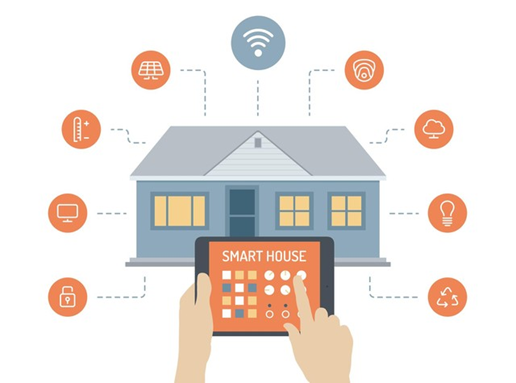
\includegraphics[width=1\textwidth]{pic10}
\caption[Ứng dụng IoT trong dân dụng ]{Ứng dụng IoT trong dân dụng}
\label{fig:pic10}
\end{figure}

Làm thế nào chúng ta có thể tận dụng thông tin thời gian thực từ rất nhiều sensor? Hãy nhìn vào ngôi nhà của chúng ta. Những phần nào trong đó có thể thông minh hóa? Ví dụ đơn giản. Tôi từng quan sát 1 hệ thống video conference cho phép người chủ nói chuyện với chú cún của mình, gọi nó đến, cho nó ăn từ xa thông qua một thiết bị thông minh. Hãy nghĩ lớn hơn nữa. Một ngôi nhà biết khi nào bạn về nhà bởi nó kết nối với một cảm biến trên xe hay smartphone của bạn. Một ngôi nhà kết nối các cảm biến báo khói, hệ thống an ninh, và thiết bị giải trí tới điện thoại của bạn. Một ngôi nhà với các cảm biến được gắn vào đường ống để có thể phát hiện ra rò rỉ trước cả khi điều đó thực sự diễn ra.

\subsection*{Ứng dụng trong y tế}
\begin{figure}[htbp!] 
\centering    
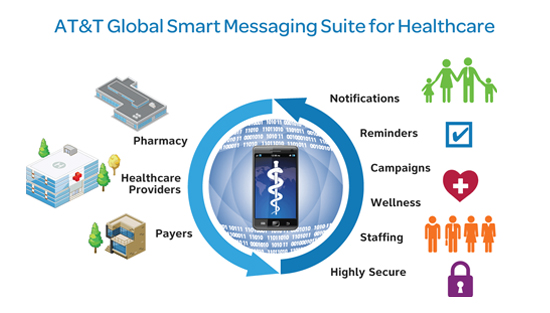
\includegraphics[width=1\textwidth]{pic11}
\caption[Ứng dụng IoT trong y tế ]{Ứng dụng IoT trong y tế}
\label{fig:pic11}
\end{figure}
Công nghệ thiết bị đeo cũng sẽ biến đổi hoàn toàn lĩnh vực chăm sóc sức khỏe theo những cách phi thường. Chúng ta đều biết rằng đồng hộ Apple Watch sẽ tích hợp một cảm biến theo dõi nhịp tim và cung cấp cho chủ của nó những ứng dụng tạo điều kiện và khuyến khích một cách sống lành mạnh. Chúng ta đã có các cảm biến gắn trong giày để theo dõi việc chạy xa đến đâu và bao nhiêu calo đã được đốt. Còn gì tiếp theo? Sẽ có một quy trình tối ưu chăm sóc sức khỏe, theo đó có những cảm biến có thể phát hiện vi khuẩn trong thiết bị, và thiết bị diệt khuẩn phát hiện virus có thể di chuyển từ bệnh nhân.


\section{Giới thiệu về các công cụ hỗ trợ phát triển ứng dụng IoT}




\section{Những yếu tố ảnh hưởng môi trường từ khí thải phương tiện giao thông}
Để hình dung được những yếu tố ảnh hưởng môi trường từ khí thải xe máy và ô tô thì chúng ta cần biết được quá trình hoạt động của xe máy và ô tô, từ đó chúng ta sẽ biết được những loại khí thải nào mà xe máy và ô tô sẽ thải ra môi trường. Qua quá trình tìm hiểu và đọc thông tin tài liệu trên mạng khí thải của xe máy và ô tô tuỳ thuộc chủ yếu vào chất lượng đốt cháy hỗn hợp xăng và không khí bên trong buồng đốt (combustion chamber) của động cơ, cũng như nồng độ các chất ô nhiễm trong khí xả phụ thuộc vào đặc điểm động cơ cũng như các thông số điều chỉnh, vận hành.

Động cơ mới và được điều chỉnh đúng cho phản ứng cháy hoàn chỉnh (complete combustion) hay phản ứng cháy thừa oxy:

\begin{center}
PTPU: Xăng + Không khí → Carbon Dioxide + Nước + Nitrogen
\end{center} 
Các phó sản (by-product) chủ yếu của phản ứng này là nước (H2O) và carbon dioxide (CO2), do đó ống thoát khí cháy (tail pipe) của một động cơ tốt thường có nước nhễu ra, dễ nhận thấy khi động cơ đang trong quá trình làm nóng máy (warm up).
Động cơ cũ hoặc không được điều chỉnh đúng cho phản ứng cháy không hoàn chỉnh (incomplete combustion) hay thiếu oxy:
\begin{center}
PTPU: Xăng + Không khí → Hydrocarbons + Nitrogen Oxides + Carbon Dioxide + Carbon Monoxide + Nước
\end{center}

Phản ứng này tạo thêm những phó sản như carbon monoxide (CO) và nitrogen oxides (NOx). Vậy chúng ta có các loại sản pham như sau:
\begin{itemize}
\item[•]CO được sinh ra khi lượng oxy đưa vào buồng đốt không đủ.
\item[•]HC được sinh ra trong quá trình đốt cháy không hoàn toàn, cũng như CO.
\item[•]NOx được sinh ra do nitơ và ôxy trong hỗn hợp không khí-nhiên liệu, khi nhiệt độ của buồng đốt tăng cao trên 1800oC.
\end{itemize}
 Nhiệt độ của buồng đốt càng cao, lượng NOx sản ra càng nhiều.
Theo lý thuyết, khi đốt cháy xăng thì chỉ sinh ra CO2 (cácbon điôxit) và H2O (hơi nước). Tuy nhiên, không phải toàn bộ xăng đều tham gia phản ứng như lí thuyết, do ảnh hưởng của các yếu tố như tỷ lệ hỗn hợp không khí-nhiên liệu, nitơ trong không khí, nhiệt độ cháy, thời gian cháy... Đó là nguyên nhân sinh ra các khí độc hại như CO, HC hoặc NOx.
Trên cơ sở thực tế, động cơ đốt trong nó chỉ sử dụng được khoảng 30-45\% nhiệt lượng để sinh công, phần còn lại bị hao hụt đi mất, do đó nó mang theo nhiệt lượng thải ra ngoài. Lượng nhiệt này thực tế đã tác động đến môi trường, làm cho nhiệt độ xung quanh những khu vực có xe máy và ô tô tăng lên. Việc đi lại trên những đoạn đường đông xe máy và ô tô thường gây cho chúng ta cảm giác nóng bức, và khó thở. Đó chính là những yếu tố khí thải đã trình bày như trên của xe máy và ô tô đã tác động đến môi trường.
Một phần nhân tố cũng đáng chú ý trong quá trình hoạt động xe máy và ô tô hoạt động đó là bụi, vì đầu vào của động cơ là xăng và không khí, mà trong xăng hiện nay thường có cặn và lượng không khí đầu vào cũng có bụi mặc dù có bộ lọc khí nhưng không thể tránh được trong quá trình sử dụng lâu dài. Một số loại phương tiện giao thông sử dụng thời gian dài, không đi bảo trì sẽ thải ra một nồng độ ô nhiễm rất lớn.
Từ những cơ sơ lý thuyết trên cho chúng ta biết được những yếu tố ảnh hưởng môi trường từ khí thải xe máy và ô tô bao gồm:
\begin{itemize}
\item[•]Khí CO2, CO, HC, NOx.
\item[•]Khói bụi.
\item[•]Yếu tố về nhiệt.
\end{itemize}








\section{Các hệ thống quan trắc hiện hữu}
\textbf{VoV giao thông:}  sử dụng hệ thống camera an ninh kết hợp với lượng phóng viên thường trực khắp thành phố để giám sát trực tiếp và cảnh báo tình trạng lưu thông trên các đoạn đường. Hệ thống có tính hiệu quả rất cao vì sử dụng CCTV giám sát tình trạng giao thông theo thời gian thực nên có góc nhìn thực tế nhất và không phục thuộc, có thể hoạt động độc lập. Tuy nhiên hệ thống vẫn có nhiều hạn chế như:
\begin{itemize}
\item[•]Vẫn chủ yếu hoạt động một cách thủ công, điều tiết và đưa ra kết quả bởi con người, chưa có áp dụng thuật toán xử lý máy tính vào công việc nhiều.
\item[•]Tốn nhiều công sức và nhân lực, cần có nhiều phóng viên trực thuộc các đoạn đường cũng như người quản lý theo dõi hệ thống camera giao thông.
\item[•]Chi phí duy trì và lắp đặt còn khá cao, và cần tốn chi phí bảo trì đắt đỏ và trình độ chuyên môn nhân viên điều hành cao, chi phí một hệ thống có thể lên tới hàng trăm tỉ. Cụ thể như hệ thống trị giá 270 tỉ VNĐ bao gồm 19 trạm giám sát camera được triển khai ở Bà Rịa - Vũng Tàu.
\end{itemize}

\begin{figure}[htbp!] 
\centering    
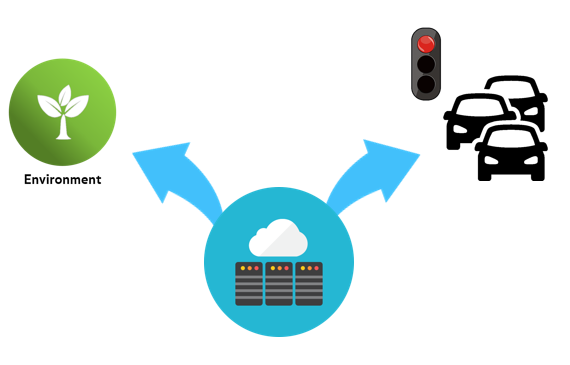
\includegraphics[width=1.0\textwidth]{pic1}
\caption[Trạm giám sát VOV Giao thông ]{Trạm giám sát VOV Giao thông}
\label{fig:pic1}
\end{figure}




\textbf{Bktraffic}  \url{http://traffic.hcmut.edu.vn} kết hợp hệ thống xe bus cùng với định vị GPS và gửi dữ liệu qua hạ tầng mạng 3G để theo dõi vị trí xe và tính toán tốc độ lưu thông trên đoạn đường xe đang lưu thông. Dự án này có hiệu quả cao vì hệ thống xe bus dày đặc và có thời gian hoạt động rộng. Tuy nhiên vẫn có những hạn chế như:
\begin{itemize}
\item[•]Vì chỉ giám sát trên xe bus nhưng nhiều trường hợp không hiệu quả khi áp dụng cho giao thông tại Việt Nam. Bởi vì đa số phương tiện giao thông ở Việt Nam là xe 2 bánh, do đó hệ thống bus di chuyển không phản ảnh được tình trạng lưu thông chung trên tuyến đường đó.
\item[•]Nhiều tuyến đường trên địa bàn thành phố mà xe bus vẫn chưa hoạt động, do vậy vẫn chưa có đủ dữ liệu cần thiết để.
\item[•]Mang tính phụ thuộc vào xe bus, vậy nên có sẽ có những trường hợp ảnh hưởng bởi hệ thống xe bus mà hệ thống sẽ không hoạt động hiệu quả được.
\end{itemize}

\begin{figure}[htbp!] 
\centering    
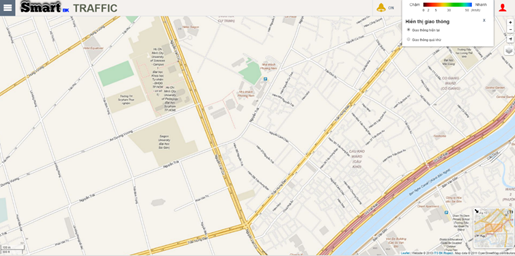
\includegraphics[width=1.0\textwidth]{pic2}
\caption[Ứng dụng Web SmartBKTraffic ]{ Ứng dụng Web SmartBKTraffic}
\label{fig:pic2}
\end{figure}




\textbf{Hệ thống quan trắc môi trường ở Hà Nội:} Thủ đô Hà Nội vừa lắp đặt hệ thống 80 trạm quan trắc. Hệ thống này có tính tương đồng với đề tài đang thực hiện. Tuy nhiên mục đích chính là để theo dõi môi trường sau sự cố bụi Thủy ngân và chưa thấy hướng ứng dụng vào hệ thống giao thông. Hơn nữa, các trạm này chiếm diện tích lắp đặt nên hạn chế khả năng triển khai số lượng lớn trên diện rộng.
\begin{figure}[htbp!] 
\centering    
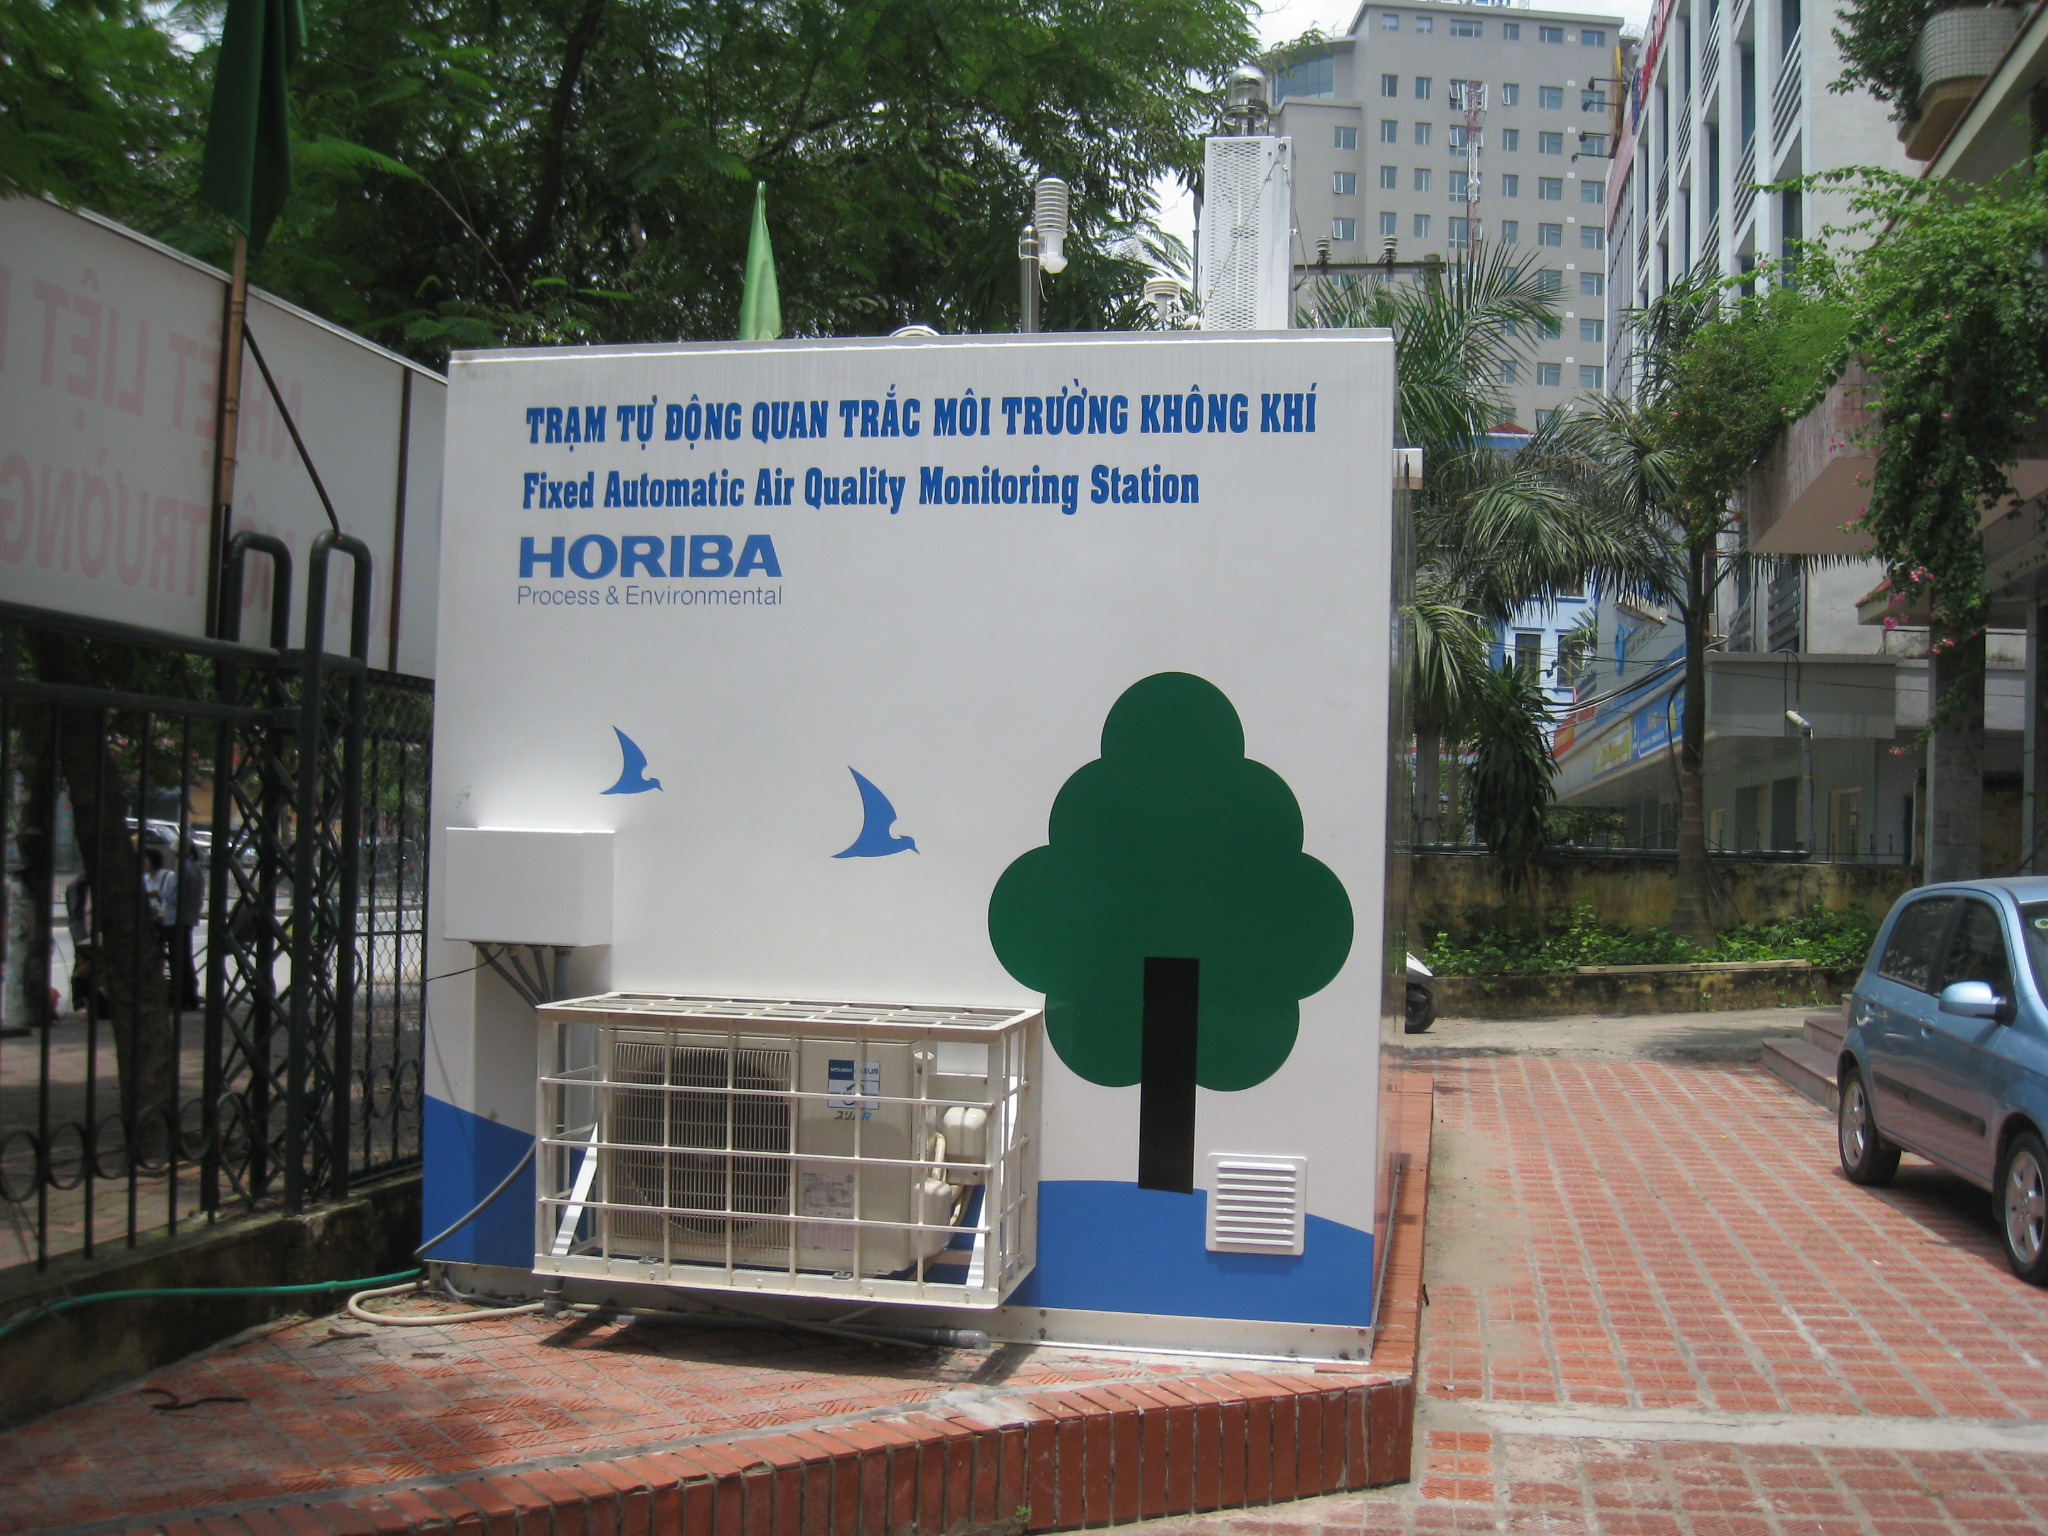
\includegraphics[width=1.0\textwidth]{pic3}
\caption[Trạm quan trắc môi trường tại Hà Nội ]{Trạm quan trắc môi trường tại Hà Nội}
\label{fig:pic3}
\end{figure}

\section{Các thiết bị phần cứng}
\subsection{Thiết bị thu thập dữ liệu}





\subsection{Các loại sensor}
%\\\\\\\\\\\\\\\\\\\\\\\\\\\\\\\\\\\\\\GP2\\\\\\\\\\\\\\\\\\\\\\\\\\\\\\\\\\\\\\\\\\\\%
\subsection*{Cảm biến bụi GP2} 
Cảm biến bụi GP2 là một bộ cảm biến chất lượng không khí quang học, được thiết kế đo những hạt bụi. Cám biến được thiết kế một điốt phát hồng ngoại và một photostransistor được sắp xếp thành đường chéo thiết bị này, cho phép nó phát hiện ánh sáng phản xạ của bụi trong không khí.  Nó đặc biệt hiệu quả trong việc phát hiện các hạt rất mịn như khói thuốc lá, và thường được sử dụng trong các hệ thống lọc không khí.

Cảm biến bụi GP2 tiêu tốn dòng rất ít (20 mA cao nhất, 11mA chế độ chạy thường), có thể hỗ trợ nguồn cung cấp lên tới 7VDC. Tín hiệu đầu ra của cảm biến là dạng tín hiệu tương tự dùng để đo mật độ bụi, với độ nhạy $0.5V/0.1mg/{m}^{3}$.

\begin{center}
\begin{figure}[htp]
\centering  
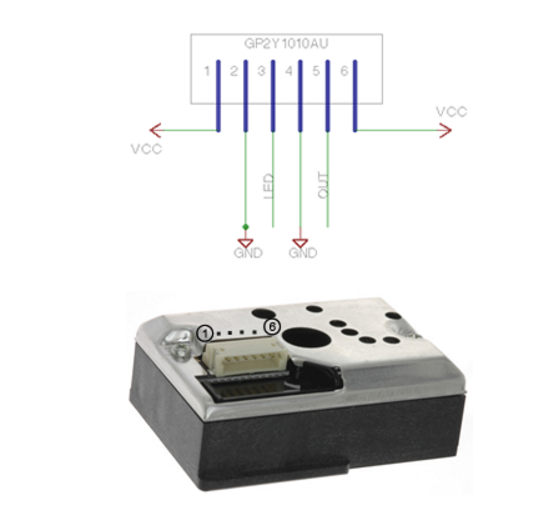
\includegraphics[width=0.4\textwidth]{gp2}
\caption[Cảm biến bụi GP2 ]{Cảm biến bụi GP2}
\label{fig:gp2}
\end{figure}
\end{center}


Thông số kỹ thuật:
\begin{itemize}
\item[•]Nguồn hoạt động: 5VDC
\item[•]Dòng tiêu thụ: 10mA
\item[•]Ngõ ra analog
\item[•]Nhiệt độ hoạt động: $-40^{o}$ $-$ $85 ^{o}$ C
\end{itemize}

Sơ đồ kết nối cảm biến bụi GP2 với Arduino

Theo hướng dẫn của tài liệu kỹ thuật, nó có tất cả gồm 6 chân đầu ra để kết nối tới thiết bị. Để có thể cảm biến bụi GP2 hoạt động với vi xử lý Arduino cần kết nối như sơ đồ luận lý sau:
\begin{center}
\begin{figure}[htp]
\centering    
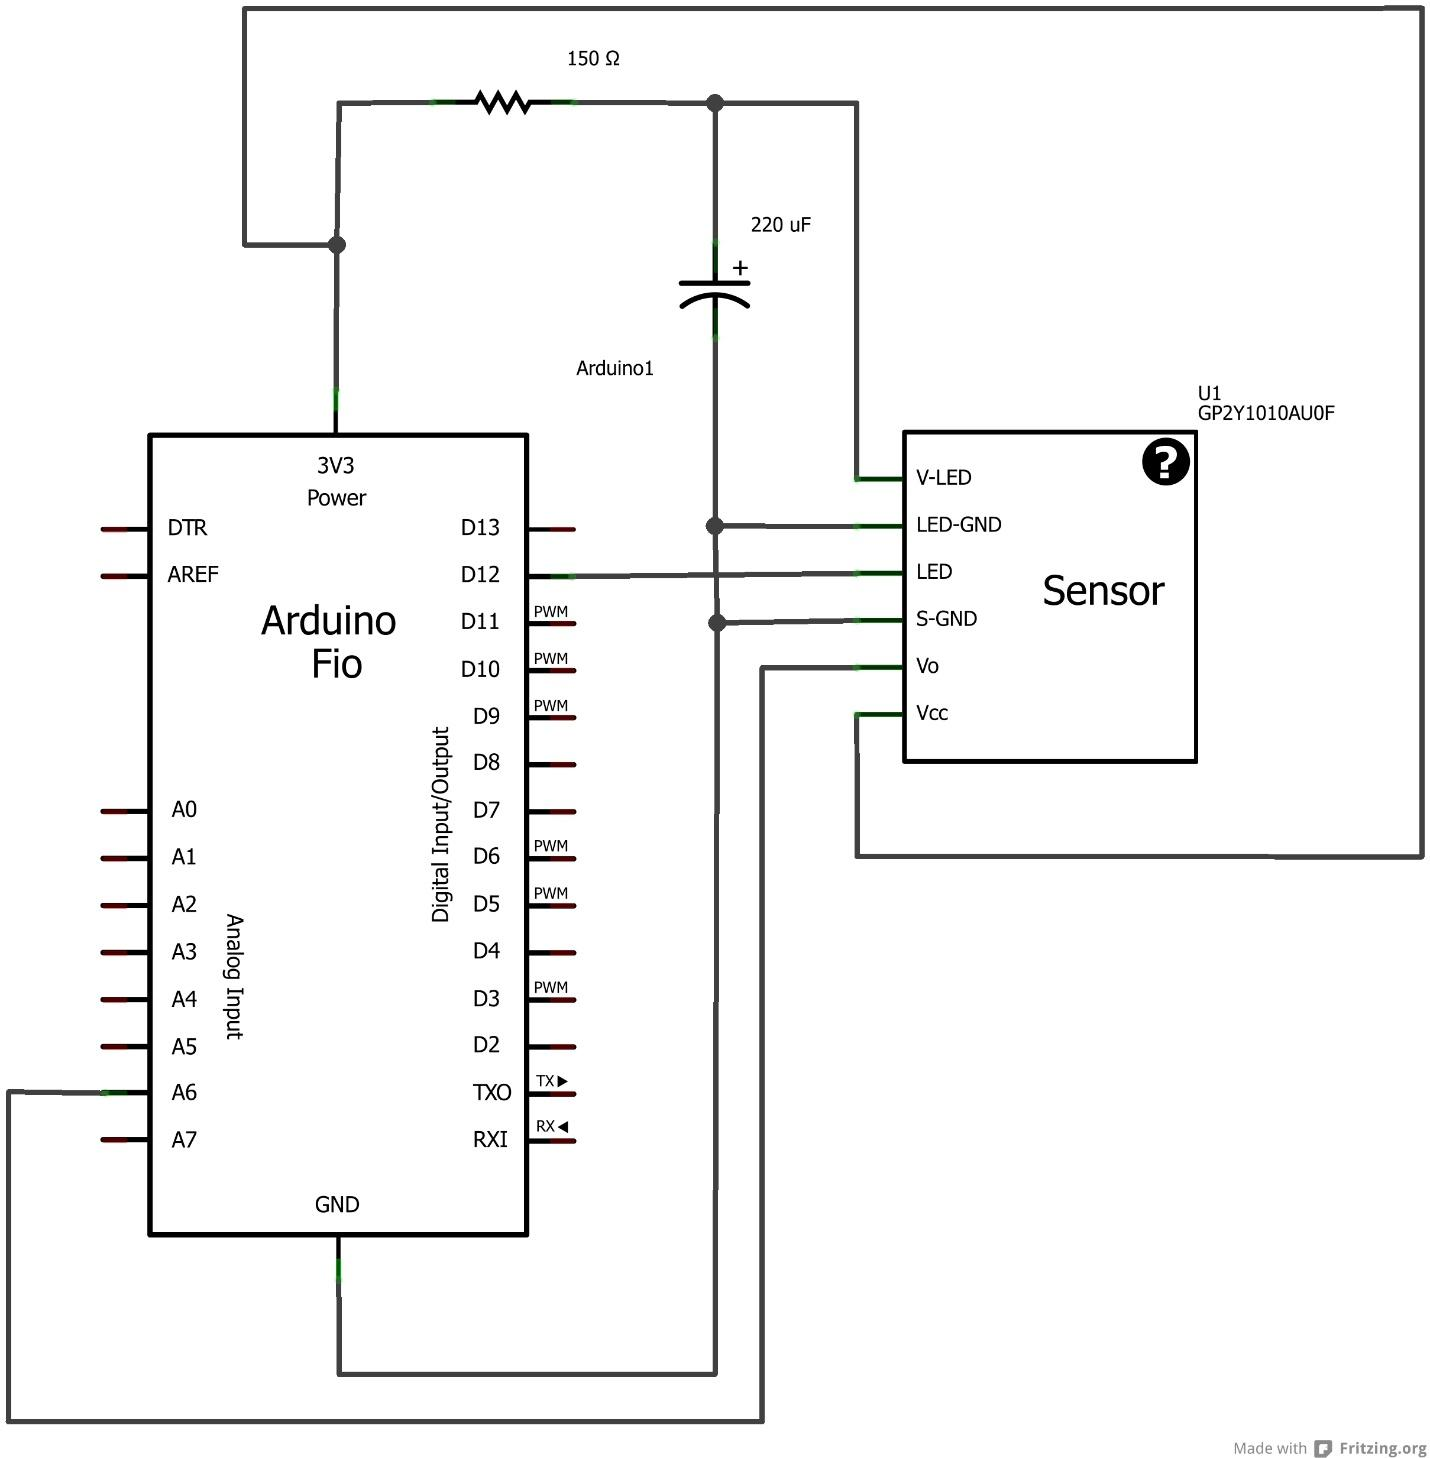
\includegraphics[width=0.7\textwidth]{sodogp2}
\caption[Sơ đồ GP2 kết nối với Arduino ]{Sơ đồ GP2 kết nối với Arduino}
\label{fig:sodogp2}
\end{figure}
\end{center}






%\\\\\\\\\\\\\\\\\\\\\\\\\\\\\\\\\\\\\\	MQ135	\\\\\\\\\\\\\\\\\\\\\\\\\\\\\\\\\\\\\\\\\\\\%
\newpage
\subsection*{Cảm biến chất lượng không khí MQ135} 
Cảm biến chất lượng không khí MQ135 thường được dùng trong các thiết bị kiểm tra chất lượng không khí bên trong cao ốc, văn phòng, thích hợp để phát hiện khí NH3, Nox, Ancol, Benzen, khói và khí CO2.Cám biến này với độ nhạy cao và thời gian đáp ứng nhanh. Tín hiệu ngõ ra dạng analog và digital. Cảm biến này có thể hoạt động ở nhiệt độ từ khoảng: $-10^{o}$C đến $50^{o}$C và tiêu thụ dòng khoảng 300mA tại 5V.

\begin{center}
\begin{figure}[htp]
\centering    
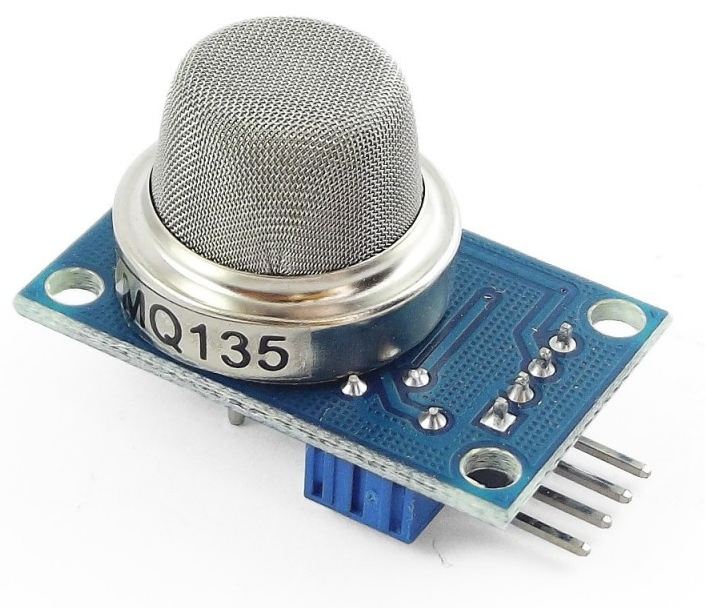
\includegraphics[width=0.7\textwidth]{mq135}
\caption[Cảm biến MQ135]{Cảm biến MQ135}
\label{fig:mq135}
\end{figure}
\end{center}

Thông số kỹ thuật:
\begin{itemize}
\item[•]Điện áp cung cấp: <=24 VDC
\item[•]Điện áp heater: 5V AC/DC
\item[•]Sử dụng chip so sánh LM393c.
\item[•]Hai tín hiệu đầu ra (digital và analog)
\item[•]Tín hiệu analog từ 0 ~ 5V.
\item[•]Dải phát hiện từ 10 đến 1000ppm
\end{itemize}
\begin{center}
\begin{figure}[htp]
\centering    
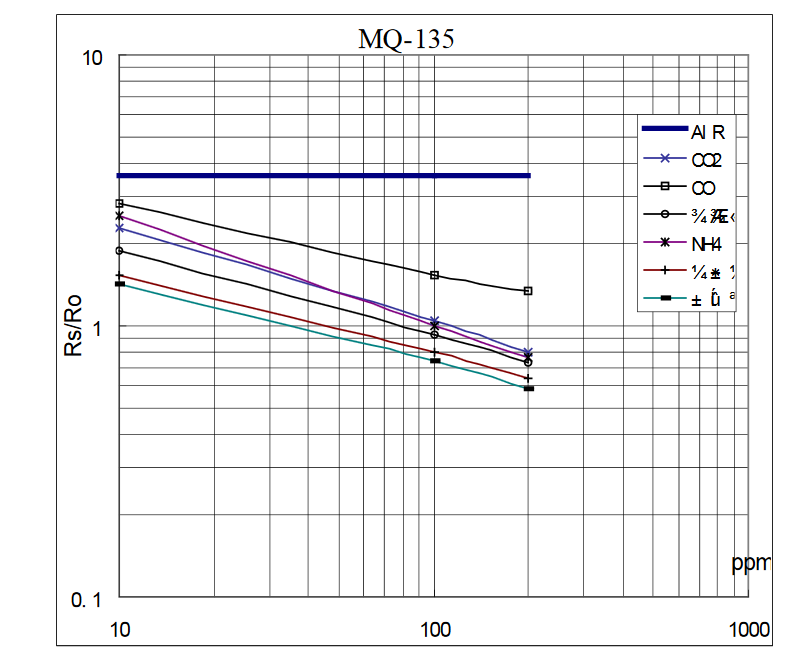
\includegraphics[width=0.7\textwidth]{mq135_mqh1}
\caption[Giản đồ chỉ sự biến đổi của Rs/Ro và giá trị ppm của MQ135]{Giản đồ chỉ sự biến đổi của Rs/Ro và giá trị ppm của MQ135}
\label{fig:mq135_mqh1}
\end{figure}
\end{center}
\begin{center}
\begin{figure}[htp]
\centering    
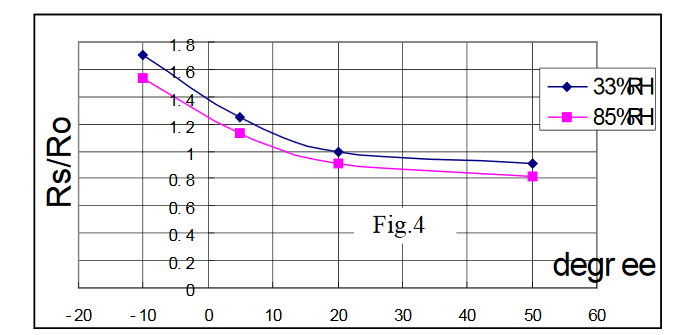
\includegraphics[width=0.7\textwidth]{mq135_mqh2}
\caption[Giản đồ chỉ sự biến đổi của Rs/Ro đối với nhiệt độ, độ ẩm]{Giản đồ chỉ sự biến đổi của Rs/Ro đối với nhiệt độ, độ ẩm}
\label{fig:mq135_mqh2}
\end{figure}
\end{center}

Giá trị chất lượng không khí(ppm) được xác định theo biểu đồ Hình \ref{fig:mq135_mqh1} giá trị này thay đổi theo sự biến đổi của giá trị Rs/Ro, theo Hình \ref{fig:mq135_mqh2} thì giá trị Rs/Ro bị ảnh hưởng bởi nhiệt độ và độ ẩm.

Để xác định được giá trị Rs/Ro từ ngõ ra analog của mạch cảm biến MQ-135 ta có công thức như sau:
\begin{center}
$\displaystyle \frac{R_{S}}{R_{L}} = \frac{V_{C}-V_{RL}}{V_{RL}}$
\end{center}

Giá trị Rs/Ro này được vi xử lý tính toán dựa trên đầu ra analog của cảm biến MQ-135 và được đưa vào thư viện mq135.h để có thể lấy được giá trị chất lượng không khí ppm theo sự thay đổi của nhiệt độ và độ ẩm của môi trường thực tế.

Thư viện mq135.h cung cấp cho chúng ta các hàm toán học đã được nhà sản xuất tính toán sẵn để có thể lấy được giá trị chất lượng không khí ppm dựa vào thay đổi của môi trường nhiệt độ và độ ẩm.



%\\\\\\\\\\\\\\\\\\\\\\\\\\\\\\\\\\\\\\	MQ07	\\\\\\\\\\\\\\\\\\\\\\\\\\\\\\\\\\\\\\\\\\\\%
\newpage
\subsection*{Cảm biến chất lượng không khí MQ07} 
Cảm biến khí CO MQ-7 có thể pháp hiện khí CO tập trung ở những nơi khác nhau từ 10 đến 1000ppm. Cám biến này với độ nhạy cao và thời gian đáp ứng nhanh. Tín hiệu ngõ ra dạng analog và digital. Cảm biến này có thể hoạt động ở nhiệt độ từ khoảng: -10C đến 50C và tiêu thụ dòng khoảng 250mA tại 5V.
\begin{center}
\begin{figure}[htp]
\centering    
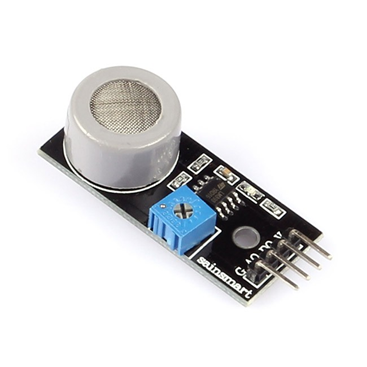
\includegraphics[width=0.7\textwidth]{mq07}
\caption[Cảm biến MQ07]{Cảm biến MQ07}
\label{fig:mq07}
\end{figure}
\end{center}

Thông số kỹ thuật:
\begin{itemize}
\item[•]Điện áp cung cấp: 3 ~ 5VDC.
\item[•]Sử dụng chip so sánh LM393 và MQ-7.
\item[•]Hai tín hiệu đầu ra (digital và analog)
\item[•]Tín hiệu analog từ 0 ~ 5V.
\item[•]Dải phát hiện từ 10 đến 1000ppm
\item[•]Kích thước: 33 x 20 x 16mm.
\end{itemize}
\begin{center}
\begin{figure}[htp]
\centering    
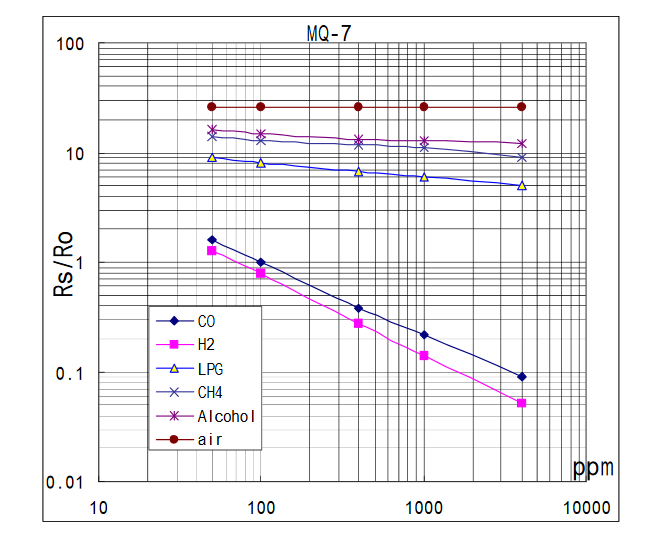
\includegraphics[width=0.7\textwidth]{mq07_mqh1}
\caption[Giản đồ chỉ sự biến đổi của Rs/Ro và giá trị ppm của MQ07]{Giản đồ chỉ sự biến đổi của Rs/Ro và giá trị ppm của MQ07}
\label{fig:mq07_mqh1}
\end{figure}
\end{center}
\begin{center}
\begin{figure}[htp]
\centering    
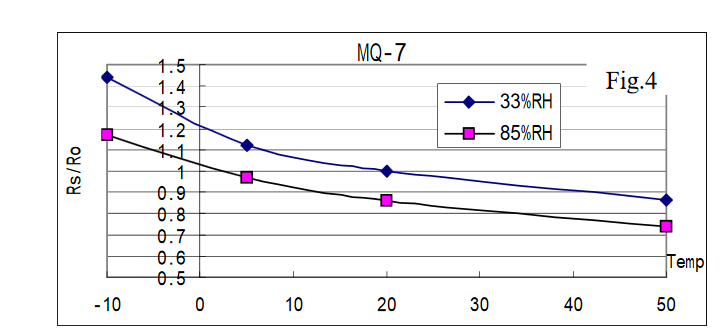
\includegraphics[width=0.7\textwidth]{mq07_mqh2}
\caption[Giản đồ chỉ sự biến đổi của Rs/Ro đối với nhiệt độ, độ ẩm]{Giản đồ chỉ sự biến đổi của Rs/Ro đối với nhiệt độ, độ ẩm}
\label{fig:mq07_mqh2}
\end{figure}
\end{center}

Giá trị chất lượng không khí(ppm) được xác định theo biểu đồ Hình \ref{fig:mq07_mqh1} giá trị này thay đổi theo sự biến đổi của giá trị Rs/Ro, theo Hình \ref{fig:mq07_mqh2} thì giá trị Rs/Ro bị ảnh hưởng bởi nhiệt độ và độ ẩm.

Để xác định được giá trị Rs/Ro từ ngõ ra analog của mạch cảm biến MQ-7 ta có công thức như sau:
\begin{center}
$\displaystyle \frac{R_{S}}{R_{L}} = \frac{V_{C}-V_{RL}}{V_{RL}}$
\end{center}

Giá trị Rs/Ro này được vi xử lý tính toán dựa trên đầu ra analog của cảm biến MQ-7 và được đưa vào thư viện mq07.h để có thể lấy được giá trị chất lượng không khí ppm theo sự thay đổi của nhiệt độ và độ ẩm của môi trường thực tế.

Thư viện mq07.h cung cấp cho chúng ta các hàm toán học đã được nhà sản xuất tính toán sẵn để có thể lấy được giá trị chất lượng không khí ppm dựa vào thay đổi của môi trường nhiệt độ và độ ẩm.






%\\\\\\\\\\\\\\\\\\\\\\\\\\\\\\\\\\\\\\	Cảm biến nhiệt độ DS18B20 IC	\\\\\\\\\\\\\\\\\\\\\\\\\\\\\\\\\\\\\\\\\\\\%
\newpage
\subsection*{Cảm biến nhiệt độ DS18B20 IC} 
Cảm biến nhiệt độ DS18B20 là cảm biến loại tín hiệu đầu ra digital đo nhiệt độ mới của hãng MAXIM với độ phân giải cao (12bit). IC được sử dụng giao tiếp 1 dây rất gọn gàng, dễ lập trình và giao tiếp nhiều DS18B20 trên cùng 1 dây. IC còn có chức năng cảnh báo nhiệt độ khi vượt ngưỡng và đặc biệt hơn là có thể cấp nguốn từ chân data.
\begin{center}
\begin{figure}[htp]
\centering    
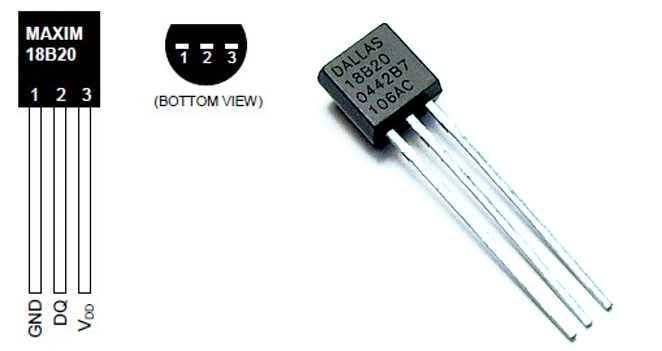
\includegraphics[width=0.7\textwidth]{ds18b20}
\caption[Cảm biến nhiệt độ DS18B20]{Cảm biến nhiệt độ DS18B20}
\label{fig:ds18b20}
\end{figure}
\end{center}
Thông số kỹ thuật:
\begin{itemize}
\item[•]Nguồn: 3-5.5V
\item[•]Dải đo nhiệt độ: -55 -125 * C
\item[•]Sai số: +-0.5 *C
\item[•]Độ phân giải: 9-12bits
\item[•]Thời gian chuyển đổi nhiệt độ: 750ms
\end{itemize}
Sơ đồ kết nối IC BS18B20 để lấy được tín hiệu data
\begin{center}
\begin{figure}[htp]
\centering    
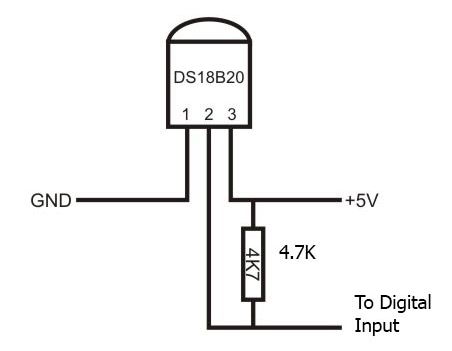
\includegraphics[width=0.7\textwidth]{ds18b20_ketnoi}
\caption[Sơ đồ kết nối DS18B20]{Sơ đồ kết nối DS18B20}
\label{fig:ds18b20_ketnoi}
\end{figure}
\end{center}	

Chân Digital input sẽ được đưa tới chân Digital input của board arduino nano, hiện tại nhà sản xuất cũng cung cấp cho lập trình viên về bộ thư viện để có thể sử dụng trong việc phát triển.

\newpage



\subsection{Mạch vi xử lý Arduino}
\subsection*{Giới thiệu về Arduino Nano}
Arduino là một board mạch vi xử lý, nhằm xây dựng các ứng dụng tương tác với nhau hoặc với môi trường được thuận lợi hơn. Phần cứng bao gồm một board mạch nguồn mở được thiết kế trên nền tảng vi xử lý AVR Atmel 8bit, hoặc ARM Atmel 32-bit. Những Model hiện tại được trang bị gồm 1 cổng giao tiếp USB, 6 chân đầu vào analog, 14 chân I/O kỹ thuật số tương thích với nhiều board mở rộng khác nhau. Đi cùng với nó là một môi trường phát triển tích hợp (IDE) chạy trên các máy tính cá nhân thông thường và cho phép người dùng viết các chương trình cho Aduino bằng ngôn ngữ C hoặc C++.

\begin{center}
\begin{figure}[htp]
\centering    
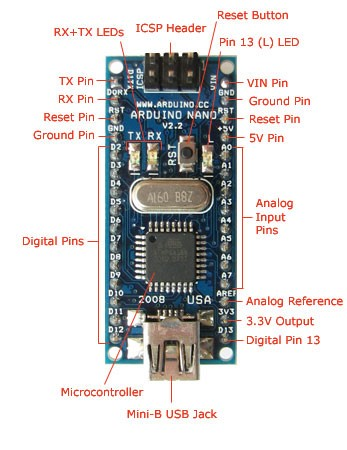
\includegraphics[width=0.4\textwidth]{arduinonano}
\caption[Mạch vi xử lý Arduino Nano]{Mạch vi xử lý Arduino Nano}
\label{fig:arduinonano}
\end{figure}
\end{center}

\newpage

\begin{center}
\begin{table}[]
\centering
\caption{Thông số của Vi xử lý Arduino}
\label{table:thongsoarduino}
\begin{tabular}{|l|l|}
\hline
Vi điều khiển                 & ATmega328 (họ 8bit)                           \\ \hline
Điện áp hoạt động             & 5VDC                                          \\ \hline
Tần số hoạt động              & 16 MHz                                        \\ \hline
Dòng tiêu thụ                 & 30mA                                          \\ \hline
Điện áp vào khuyên dùng       & 7-12 VDC                                      \\ \hline
Điện áp vào giới hạn          & 6-20 VDC                                      \\ \hline
Số chân Digital I/O           & 14 (6 chân PWM)                               \\ \hline
Số chân Analog                & 8 (độ phân giải 10bit)                        \\ \hline
Dòng,tối đa trên mỗi chân I/O & 40 mA                                         \\ \hline
Dòng ra tối đa (5V)           & 500 mA                                        \\ \hline
Dòng ra tối đa (3.3V)         & 50 mA                                         \\ \hline
Bộ nhớ flash                  & 32 KB (ATmega328) với 2KB dùng bởi bootloader \\ \hline
SRAM                          & 2 KB (ATmega328)                              \\ \hline
EEPROM                        & 1 KB (ATmega328)                              \\ \hline
Kích thước                    & 1.85cm x 4.3cm                                \\ \hline
\end{tabular}
\end{table}
\end{center}


\subsection*{Lập trình cho Arduino Nano}
Arduino Nano sử dụng chương trình Arduino IDE để lập trình, và ngôn ngữ lập trình cho Arduino cũng tên là Arduino (được xây dựng trên ngôn ngữ C). 

Arduino IDE là môi trường phát triển tích hợp (IDE) của Arduino là một ứng dụng cross-platform (nền tảng) được viết bằng Java, và từ IDE này sẽ được sử dụng cho ngôn ngữ lập trình xử lý (Processing programming language) và project Wiring. Nó được thiết kế để dành cho những người mới tập tành làm quen với lĩnh vực phát triển phần mềm. Nó bao gồm một chương trình code editor với các chức năng như đánh dấu cú pháp, tự động brace matching, và tự động canh lề, cũng như compile và upload chương trình lên board chỉ với 1 cú click chuột. Một chương trình hoặc code viết cho Arduino được gọi là một sketch.

\newpage

\begin{center}
\begin{figure}[htp]
\centering    
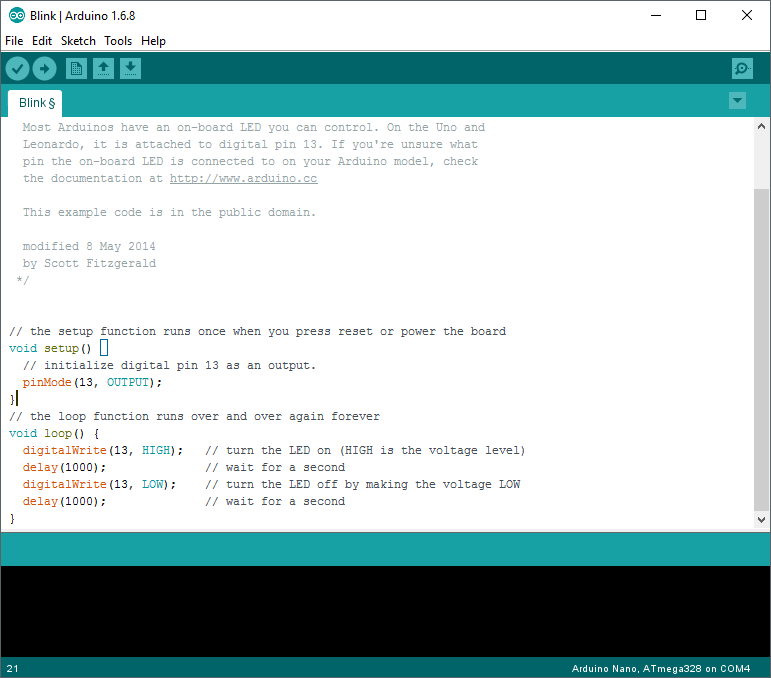
\includegraphics[width=1\textwidth]{arduinonano_ide}
\caption[Môi trường phát triển của Arduino]{Môi trường phát triển của Arduino}
\label{fig:arduinonano_ide}
\end{figure}
\end{center}

Các chương trình Arduino được viết bằng C hoặc C++. Arduino IDE đi kèm với một thư viện phần mềm được gọi là "Wiring", từ project Wiring gốc, có thể giúp các thao tác input/output được dễ dàng hơn. Người dùng chỉ cần định nghĩa 2 hàm để tạo ra một chương trình vòng thực thi (cyclic executive) có thể chạy được:
\begin{itemize}
\item[•]Setup(): hàm này chạy mỗi khi khởi động một chương trình, dùng để thiết lập
các cài đặt
\item[•]Loop(): hàm này được gọi lặp lại cho đến khi tắt nguồn board mạch
\end{itemize}

	\begin{lstlisting}[caption=Đoạn code nháy đèn căn bản]
// the setup function runs once
void setup() {
  // initialize digital pin 13 as an output.
  pinMode(13, OUTPUT);
}

// the loop function runs forever
void loop() {
  // turn the LED on (HIGH is the voltage level)
  digitalWrite(13, HIGH);   
  // wait for a second
  delay(1000);    
  // turn the LED off by making the voltage LOW          
  digitalWrite(13, LOW);    
  // wait for a second
  delay(1000);              
}

	\end{lstlisting}







%\\\\\\\\\\\\\\\\\\\\\\\\\\\\\\\\\\\\\\	SIM800L	\\\\\\\\\\\\\\\\\\\\\\\\\\\\\\\\\\\\\\\\\\\\%
\subsection{Module SIM800L}
\subsection*{Giới thiệu về Sim800L}
Thừa kế các chức năng từ các thế hệ modile sim trước như sim900, Module GSM sim 800L có khả năng nhắn tin SMS, nghe gọi, GPRS, … như một điện thoại nhưng có kích thuốc nhỏ nhất trong các loại module SIM (25 mm x 22 mm). Điều khiển module sử dụng các bộ tập lệnh AT dễ dàng, chân kết nối dùng rào đực thông dụng chuẩn 100mil.
Thông số kỹ thuật:
\begin{itemize}

\item[•]Nguồn cấp: 3.7 – 4.2 VDC, có thể sử dụng với nguồn dòng thấp từ 500mAh trở lên, nhưng để sim hoạt động đảm bảo thì dòng đủ 1A là được khuyến khích dùng hơn.
\item[•]Khe cắm SIM: MICROSIM
\item[•]Dòng khi ở chế độ chờ: 10mA
\item[•]Dòng khi hoạt động: 100mA đến 1A
\item[•]Hỗ trợ 4 băng tần phổ biến: GSM 850, EGSM 900, DCS 1800, PCS 1900.
\item[•]Nhiệt độ hoạt động: -40 C ~ 85 C
\item[•]Tốc độ truyền downlink/uplink: cao nhất 85.6 kbps
\item[•]Tốc độ UART hỗ trợ: 1200bps đến 125200bps
\end{itemize}

Chức năng các chân của module Sim800L
\begin{center}
\begin{figure}[htp]
\centering    
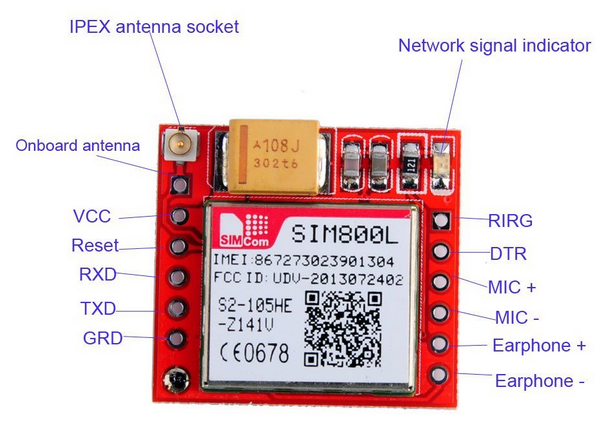
\includegraphics[width=0.7\textwidth]{sim800l}
\caption[Sơ đồ module sim800l]{Sơ đồ module sim800l}
\label{fig:sim800l}
\end{figure}
\end{center}	

\begin{itemize}
\item[•]TXD: chân truyền UART TX
\item[•]RXD: chân nhận UART RX
\item[•]DTR: chân UART DTR, thường ít xài.
\item[•]SPKP, SPKN: ngõ ra âm thanh, nối với loa để phát âm thanh.
\item[•]MICP, MICN: ngõ vào âm thanh, phải găn thêm micro để thu âm thanh.
\item[•]Reset: chân khởi động lại SIM800L
\item[•]RING: báo cuộc gọi đến
\item[•]GND: chân Mass, cấp 0v.
\end{itemize}

%/////////////////////////////////////////////////////////////////////////AT SIM 800L
\newpage
\subsection*{Một số tập lệnh AT của module Sim800L dùng trong đề tại luận văn}


 AT+CBC: trả về kết quả dung lượng pin hiện tại.
\begin{table}[htp]
\label{table:at+cbc}
\begin{tabular}{|l|l|}
\hline
Lệnh AT & AT+CBC \\ \hline
Kết quả  & 
+ CBC: <bcs>, <bcl>, <voltage> \\
&OK \\
& \\
& Với các thông số \\
& \hspace{0.5cm} <bcs>: \\
& \hspace{2cm} • 0: Mạch không phải trạng thái đang sạc. \\
& \hspace{2cm} • 1: Mạch đang trong trạng thái sạc. \\
& \hspace{2cm} • 2: Mạch đã sạc xong. \\
& \hspace{0.5cm} <bcl>: giá trị \% dung lượng pin: 1 …100 \%. \\
& \hspace{0.5cm} <voltage>: Giá trị nguồn đầu vào của module sim (mV) \\\hline
\end{tabular}
\caption[Tập lệnh AT+CBC: kết quả dung lượng pin hiện tại]{Tập lệnh AT+CBC}
\end{table}



 AT+ CCLK trả về giá trị thời gian của module sim
\begin{table}[htp]
\label{table:at+cclk}
\begin{tabular}{|l|l|}
\hline
Lệnh AT & AT+CCLK \\ \hline
Kết quả  & 
+ CBC: <time> \\
&OK \\
& \\
& Với các thông số \\
& \hspace{0.5cm}<time>: là một dạng chuỗi String, chuỗi String này được format\\
& \hspace{0.5cm} dưới dạng $yy/MM/dd, hh:mm:ss+-zz$ \\\hline
\end{tabular}

\caption[Tập lệnh AT+CCLK: trả về giá trị thời gian của module sim]{Tập lệnh AT+CCLK}
\end{table}



AT+CSTT cài đặt các thông số APN, USER NAME, PASSWORD cho Sim
\begin{table}[htp]
\label{table:at+cstt}
\begin{tabular}{|l|l|}
\hline
Lệnh AT & AT+CSTT= <apn>,<user>,<password> \\ 
& \\
& \hspace{0.5cm}<apn> Địa điểm truy cập GPRS\\
& \hspace{0.5cm}<user> Tên đăng nhập\\
& \hspace{0.5cm}<pass> Mật khẩu đăng nhập\\
& \\
& 3 thông số trên được cung cấp theo từng nhà mạng của mỗi sim khi \\
& được gắn vào module sim, mục đích dùng để xác nhận việc truy cập \\
& GPRS vào các nhà mạng.\\
& Ví dụ thông số của nhà mạng vinaphone: <m3-world>,<mms>,<mms> \\\hline
Kết quả  &+ OK \\\hline
\end{tabular}

\caption[Tập lệnh AT+CSTT: cài đặt các thông số APN, USER NAME, PASSWORD cho Sim]{Tập lệnh AT+CSTT}
\end{table}





AT+CIFSR: Lấy thông tin địa chỉ IP của moduleSIM
\begin{table}[htp]
\label{table:AT+CIFS}
\begin{tabular}{|l|l|}
\hline
Lệnh AT & AT+CIFSR \\ \hline
Kết quả  & 
<IP address> \\
& \\
& <IP address>: địa chỉ IP được gắn sau khi tham gia vào GPRS.\\\hline
\end{tabular}

\caption[Tập lệnh AT+CIFSR: lấy thông tin địa chỉ IP của moduleSIM]{Tập lệnh AT+CIFSR}
\end{table}




AT+CIPSTART: thiết lập kết nối TCP hoặc UDP
\begin{table}[htp]
\label{table:AT+CIPSTART}
\begin{tabular}{|l|l|}
\hline
Lệnh AT & AT+CIPSTART=”TCP”,”192.168.0.1”,”80” \\ 
& Kết nối tới địa chỉ 192.168.0.1 tại cổng 80 với giao thức TCP.\\
& \\
& AT+CIPSTART=”UDP”,”192.168.0.1”,”8888” \\ 
& Kết nối tới địa chỉ 192.168.0.1 tại cổng 8888 với giao thức UDP.\\ \hline
Kết quả  &+ OK \\
& \\
& CONNECT OK\\\hline
\end{tabular}

\caption[Tập lệnh AT+CIPSTART: thiết lập kết nối TCP hoặc UDP]{Tập lệnh AT+CIPSTART}
\end{table}


AT+CDNSGIP: được dùng để phân giải DNS của một tên miền, nó được sử dụng cho việc thiếp lập kết nối TCP/UCP thông qua tên miền bằng câu lệnh “AT+CIPSTART=<mode>,<domain name>, <port>”, và sau đó người dùng có thể gửi dữ liệu đến máy chủ thông qua câu lệnh AT+CIPSEND.
\begin{table}[htp]
\label{table:AT+CDNSGIP}
\begin{tabular}{|l|l|}
\hline
Lệnh AT & AT+CDNSGIP=<domain name> \\ 
& \\
& <domain name>: Tên miền muốn phân giải DNS, \\

& ví dụ như AT+CDNSGIP= “www.codingyourfuture.com “\\ \hline
Kết quả  &OK \\
&+ CDNSGIP:\\
&1,”www.codingyourfuture.com”,”113.173.153.194”,”119.75.217.56”\\\hline
\end{tabular}

\caption[Tập lệnh AT+CDNSGIP: phân giải DNS tên miền]{Tập lệnh AT+CDNSGIP}
\end{table}












AT+CIPSEND: gửi dữ liệu thông qua giao thức kết nối TCP/UCP
\begin{table}[htp]
\label{table:AT+CIPSEND}
\begin{tabular}{|l|l|}
\hline
Lệnh AT & AT+CIPSEND=<length> \\ 
& \\
& <length>: độ dài dữ liệu muốn gửi.\\\hline
Kết quả  & >  \\ \hline
Lệnh AT & Dữ liệu muốn gửi đi \\ \hline
Kết quả  & OK  \\ \hline
\end{tabular}

\caption[Tập lệnh AT+CIPSEND: gửi dữ liệu qua giao thức TCP/UCP]{Tập lệnh AT+CIPSEND}
\end{table}







\newpage

\subsection*{Quá trình kết nối giao thức TCP tới máy chủ thông qua GPRS}
Quá trình kết nối tới máy chủ thông qua giao thức TCP được thực hiện dựa trên mô hình máy trạng thái như sau:


\begin{center}
\begin{figure}[htpd]
\centering    
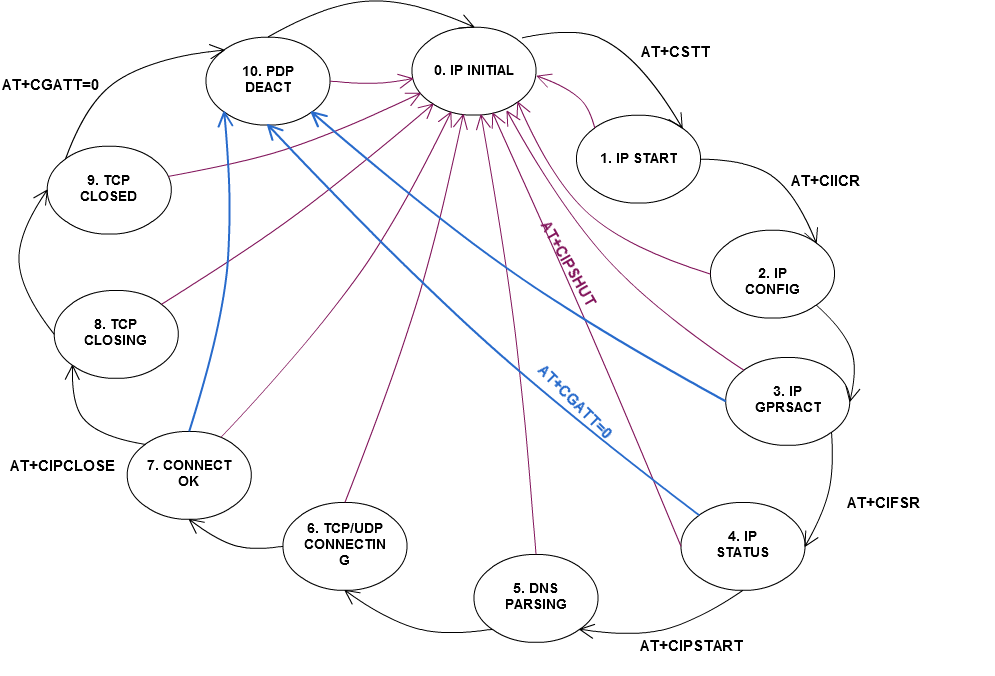
\includegraphics[width=0.9\textwidth]{sim800_status}
\caption[Sơ đồ trạng thái GPRS cho đơn kết nối]{Sơ đồ trạng thái GPRS cho đơn kết nối}
\label{fig:sim800_status}
\end{figure}
\end{center}

Để gửi được dữ liệu đến máy chủ cần phải thiết lập được kết nối TCP từ module SIM800 đến máy chủ thông qua 11 trạng thái như Hình \ref{fig:sim800_status}. Đến trạng thái 7 (CONNET OK) chúng ta đã giữ được kết nối TCP tới máy chủ và tại trạng thái này dùng lệnh AT+CIPSEND để thực hiện việc gửi gói dữ liệu lên cho máy chủ.

Gói dữ liệu được gửi theo phương thức GET, bên máy chủ phải hỗ trợ được phương thức GET này và định nghĩa rõ ràng các kiểu và số lượng dữ liệu gửi lên. 

Dữ liệu sensor node gửi lên cho máy chủ gồm các dữ liệu sau:
\begin{table}[]
\centering
\label{table:sensornode_api}
\begin{tabular}{|l|l|l|l|l|l|}
\hline
\begin{tabular}[c]{@{}l@{}}NODE\\ ID\end{tabular} & \begin{tabular}[c]{@{}l@{}}Giá trị CO\\ (ppm)\end{tabular} & \begin{tabular}[c]{@{}l@{}}Giá trị \\ nhiệt độ \\ (Độ C)\end{tabular} & \begin{tabular}[c]{@{}l@{}}Giá trị\\ độ bụi\\ (ppm)\end{tabular} & \begin{tabular}[c]{@{}l@{}}Giá trị chất\\ lượng không \\ khí (ppm)\end{tabular} & \begin{tabular}[c]{@{}l@{}}Giá trị dung\\ lượng pin (\%)\end{tabular} \\ \hline
\end{tabular}
\end{table}














\newpage
\subsection{Pin năng lượng mặt trời}
Pin năng lượng mặt trời (pin mặt trời/pin quang điện) là thiết bị giúp chuyển hóa trực tiếp năng lượng ánh sáng mặt trời (quang năng) thành năng lượng điện (điện năng) dựa trên hiệu ứng quang điện. Hiệu ứng quang điện là khả năng phát ra điện tử (electron) khi được ánh sáng chiếu vào của vật chất.

Tấm pin mặt trời, những tấm có bề mặt lớn thu thập ánh nắng mặt trời và biến nó thành điện năng, được làm bằng nhiều tế bào quang điện có nhiệm vụ thực hiện quá trình tạo ra điện từ ánh sáng mặt trời.



\begin{center}
\begin{figure}[htp]
\centering    
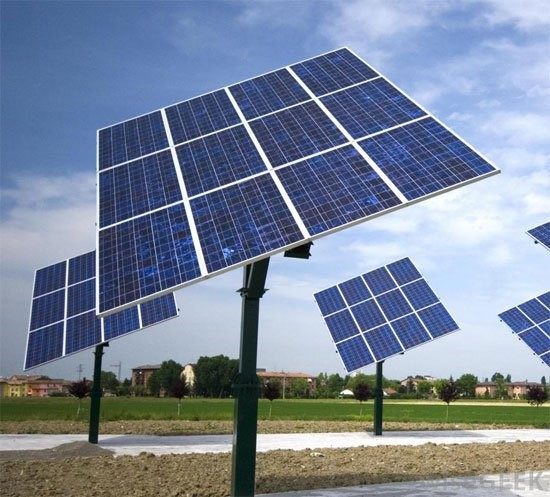
\includegraphics[width=0.7\textwidth]{solarpanel}
\caption[Tấm pin năng lượng mặt trời]{Tấm pin năng lượng mặt trời}
\label{fig:solarpanel}
\end{figure}
\end{center}

\subsection*{Chất bán dẫn Silicon}
Silicon được biết đến là một chất bán dẫn. "Chất bán dẫn là vật liệu trung gian giữa chất dẫn điện và chất cách điện. Chất bán dẫn hoạt động như một chất cách điện ở nhiệt độ thấp và có tính dẫn điện ở nhiệt độ phòng". Với tính chất như vậy, silicon là một thành phần quan trọng trong cấu tạo của pin năng lượng mặt trời.

Silicon tuy có mức dẫn điện hạn chế nhưng nó có cấu trúc tinh thể rất phù hợp cho việc tạo ra chất bán dẫn. Nguyên tử silicon cần 4 electron để trung hòa điện tích nhưng lớp vỏ bên ngoài một nguyên tử silicon chỉ có một nửa số electron cần thiết nên nó sẽ bám chặt với các nguyên tử khác để tìm cách trung hòa điện tích.

Để tăng độ dẫn điện của silicon, các nhà khoa học đã “tạp chất hóa” nó bằng cách kết hợp nó với các vật liệu khác. Quá trình này được gọi là “doping” và silicon pha tạp với các tạp chất tạo ra nhiều electron tự do và lỗ trống. Một chất bán dẫn silicon có hai phần, mỗi phần được pha tạp với một loại vật liệu khác. Phần đầu tiên được pha với phốt pho, phốt pho cần 5 electron để trung hòa điện tích và có đủ 5 electron trong vỏ của nó. Khi kết hợp với silicon, một electron sẽ bị dư ra. Electron đặc trưng cho điện tích âm nên phần này sẽ được gọi là silicon loại N (điện cực N). Để tạo ra silicon loại P (điện cực P), các nhà khoa học kết hợp silicon với boron. Boron chỉ cần 3 electron để trung hòa điện tích và khi kết hợp với silicon sẽ tạo ra những lỗ trống cần được lấp đầy bởi electron.


\begin{center}
\begin{figure}[htp]
\centering    
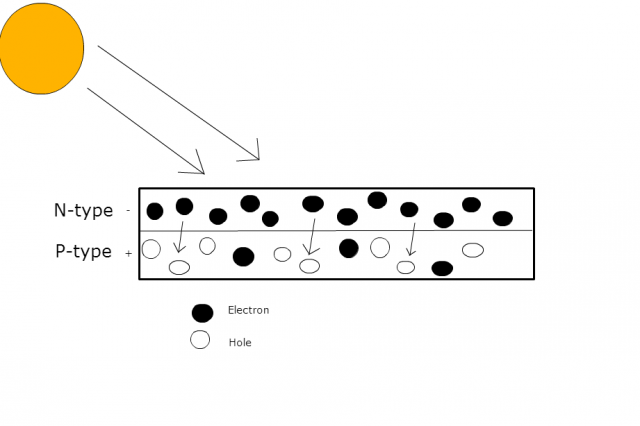
\includegraphics[width=0.7\textwidth]{solarpanel_hinhthanhdientich}
\caption[Tấm pin năng lượng mặt trời]{Tấm pin năng lượng mặt trời}
\label{fig:solarpanel_hinhthanhdientich}
\end{figure}
\end{center}


Khi chất bán dẫn silicon tiếp xúc với năng lượng, các electron tự do ở điện cực N sẽ di chuyển sang để lấp đầy các lỗ trống bên điện cực P. Sau đó, các electron từ điện cực N và điện cực P sẽ cùng nhau tạo ra điện trường. Các tế bào năng lượng mặt trời sẽ trở thành một diode, cho phép electron di chuyển từ điện cực P đến điện cực N, không cho phép di chuyển ngược lại.

Tất nhiên, để kích hoạt quá trình cần có năng lượng tiếp xúc với các tế bào silicon. Ánh sáng mặt trời bao gồm các hạt rất nhỏ gọi là photon được tỏa ra từ mặt trời, các hạt nhỏ năng lượng có thể tiếp xúc với các tế bào năng lượng mặt trờivà nới lỏng liên kết của các electron ở điện cực N. Sự di chuyển của các elentron tự do từ điện cực N tới điện cực P tạo ra dòng điện.





\subsection*{Hiệu suất của pin mặt trời}
Các công nghệ biến ánh sáng mặt trời thành điện hiện tại vẫn kém hiệu quả. Các tấm pin mặt trời chưa thể hấp thụ toàn bộ năng lượng của ánh sáng mặt trời. Nói chung, những tế bào năng lượng mặt trời tốt nhất hiện tại chỉ có thể chuyển 25\% năng lượng mà nó nhận được thành điện. Tại sao vậy? Thực tế là ánh sáng mặt trời, như tất cả các loại ánh sáng khác, bao gồm một quang phổ với các bước sóng khác nhau, mỗi bước sóng có một cường độ khác nhau. Có những bước sóng quá yếu không thể giải phóng các electron còn một số bước sóng lại quá mạnh với silicon.


\subsection*{Tấm pin mặt trời được dùng cho đề tài}

Pin năng lượng mặt trời Poly 5V /220 mA

\begin{center}
\begin{figure}[htp]
\centering    
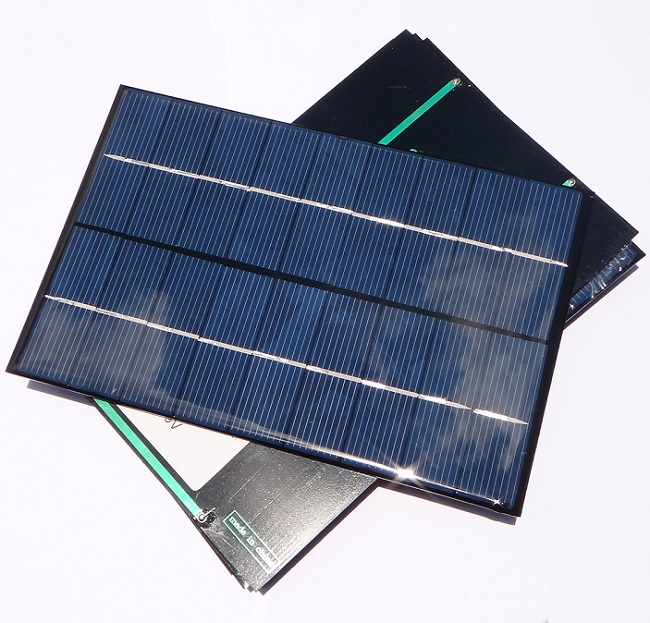
\includegraphics[width=0.6\textwidth]{solarpanel_real}
\caption[Pin năng lượng mặt trời Poly 5V /220 mA]{Pin năng lượng mặt trời Poly 5V /220 mA}
\label{fig:solarpanel_real}
\end{figure}
\end{center}


Với kích thước: 100x80x2mm
Nguồn đầu ra: 5V
Dòng tối đa cung cấp được là 220mA





\section{Kiến thức căn bản về ứng dụng web - di động và xây dựng Server}

\subsection{Giao thức TCP}
%TODO: ref https://vi.wikipedia.org/wiki/TCP
TCP (Transmission Control Protocol - "Giao thức điều khiển truyền vận") là một trong các giao thức cốt lõi của bộ giao thức TCP/IP. Sử dụng TCP, các ứng dụng trên các máy chủ được nối mạng có thể tạo các "kết nối" với nhau, mà qua đó chúng có thể trao đổi dữ liệu hoặc các gói tin. Giao thức này đảm bảo chuyển giao dữ liệu tới nơi nhận một cách đáng tin cậy và đúng thứ tự. TCP còn phân biệt giữa dữ liệu của nhiều ứng dụng (chẳng hạn, dịch vụ Web và dịch vụ thư điện tử) đồng thời chạy trên cùng một máy chủ.

TCP hỗ trợ nhiều giao thức ứng dụng phổ biến nhất trên Internet và các ứng dụng kết quả, trong đó có WWW, thư điện tử và Secure Shell.

Trong bộ giao thức TCP/IP, TCP là tầng trung gian giữa giao thức IP bên dưới và một ứng dụng bên trên. Các ứng dụng thường cần các kết nối đáng tin cậy kiểu đường ống để liên lạc với nhau, trong khi đó, giao thức IP không cung cấp những dòng kiểu đó, mà chỉ cung cấp dịch vụ chuyển gói tin không đáng tin cậy. TCP làm nhiệm vụ của tầng giao vận trong mô hình OSI đơn giản của các mạng máy tính.

Các ứng dụng gửi các dòng gồm các byte 8-bit tới TCP để chuyển qua mạng. TCP phân chia dòng byte này thành các đoạn (segment) có kích thước thích hợp (thường được quyết định dựa theo kích thước của đơn vị truyền dẫn tối đa (MTU) của tầng liên kết dữ liệu của mạng mà máy tính đang nằm trong đó). Sau đó, TCP chuyển các gói tin thu được tới giao thức IP để gửi nó qua một liên mạng tới mô đun TCP tại máy tính đích. TCP kiểm tra để đảm bảo không có gói tin nào bị thất lạc bằng cách gán cho mỗi gói tin một "số thứ tự" (sequence number). Số thứ tự này còn được sử dụng để đảm bảo dữ liệu được trao cho ứng dụng đích theo đúng thứ tự. Mô đun TCP tại đầu kia gửi lại "tin báo nhận" (acknowledgement) cho các gói tin đã nhận được thành công; một "đồng hồ" (timer) tại nơi gửi sẽ báo time-out nếu không nhận được tin báo nhận trong khoảng thời gian bằng một round-trip time (RTT), và dữ liệu (được coi là bị thất lạc) sẽ được gửi lại. TCP sử dụng checksum (giá trị kiểm tra) để xem có byte nào bị hỏng trong quá trình truyền hay không; giá trị này được tính toán cho mỗi khối dữ liệu tại nơi gửi trước khi nó được gửi, và được kiểm tra tại nơi nhận.

\subsection{Căn bản về RESTful Web services}

\textbf{Tổng quan về REST – Representational State Transfer}

REST là một kiểu kiến trúc dựa trên các tiêu chuẩn web và giao thức HTTP. REST được mô tả đầu tiên bởi Roy Fielding trong luận văn tiến sĩ của ông vào năm 2000.

Trong một kiến trúc REST thì tất cả mọi thứ là một nguồn tài nguyên. Một nguồn tài nguyên được truy cập thông qua một giao diện phổ biển dựa trên các phương pháp tiêu chuẩn HTTP.

Một kiến trúc REST thường có một REST server cung cấp truy cập đến các nguồn tài nguyên và một Rest client truy cập và trình sửa các tài nguyên đó.

REST cho phép các nguồn tài nguyên biểu diễn dưới nhiều kiểu khác nhau như Text, XML, JSON … Rest client có thể yêu cầu một kiểu biểu diễn cụ thể thông qua giao thức HTTP.

\textbf{Các phương thức HTTP}

Các phương thức PUT, GET, POST và DELETE thường được sử dụng trong kiến trúc REST

• \textbf{GET} định nghĩa một truy cập đọc nguồn tài nguyên mà không có tác dụng phụ. Nguồn tài nguyên không bao giờ thay đổi thông qua một yêu cầu GET.

• \textbf{PUT} dùng để tạo một tài nguyên mới.

• \textbf{DELETE} loại bỏ các nguồn tài nguyên.

• \textbf{POST} cập nhật một nguồn tài nguyên hiện có hoặc tạo ra một nguồn tài nguyên mới.

\textbf{RESTful webservice}

Một RESTful webservice được dựa trên các phương thức HTTP và các khái niệm về REST. Một RESTful webservice thường xác định URI cơ sở cho các dịch vụ, hỗ trợ các kiểu MIME (XML, Text, JSON,…) và tập các hoạt động (POST, GET, PUT, DELETE) đều được hỗ trợ.

\textbf{JSON (JavaScript Object Notation)}

Là một định dạng hoán vị dữ liệu nhanh. Chúng dễ dàng cho chúng ta đọc và viết. Dễ dàng cho thiết bị phân tích và phát sinh. Chúng là cơ sở dựa trên tập hợp của Ngôn Ngữ Lập Trình JavaScript, tiêu chuẩn ECMA-262 phiên bản 3 – tháng 12 năm 1999. JSON là một định dạng kiểu text mà hoàn toàn độc lập với các ngôn ngữ hoàn chỉnh, thuộc họ hàng với các ngôn ngữ họ hàng C, gồm có C, C++, C, Java, JavaScript, Perl, Python, và nhiều ngôn ngữ khác. Những đặc tính đó đã tạo nên JSON một ngôn ngữ hoán vị dữ liệu lý tưởng.

JSON được xây dựng trên 2 cấu trúc:

• Là tập hợp của các cặp tên và giá trịname – value. Trong những ngôn ngữ khác nhau, đây được nhận thấy như là một đối tượng (object), sự ghi (record), cấu trúc (struct), từ điển (dictionary), bảng băm (hash table), danh sách khóa (keyed list), hay mảng liên hợp.

• Là một tập hợp các giá trị đã được sắp xếp. Trong hầu hết các ngôn ngữ, nó được nhận thấy như là một mảng, vector, list hay là một dãy sequence.


\begin{figure}[H]
	\centering    
	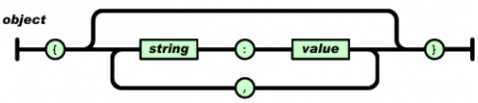
\includegraphics[width=1.0\textwidth]{json0}
	\caption[Cấu trúc của một đối tượng JSON]{Cấu trúc của một đối tượng JSON}
	\label{fig: json0}
\end{figure}

Một đối tượng là một tập hợp của các cặp tên/giá trị (name/value). Một đối tượng bắt đầu bởi dấu “{“ và kết thúc với dấu “}”. Từng tên được theo sau bởi dấu “:” và các cặp tên/giá trị được tách ra bởi dấu “,”.

\begin{figure}[H]
	\centering    
	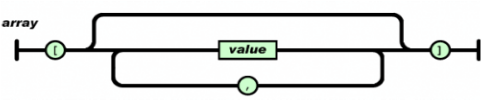
\includegraphics[width=1.0\textwidth]{json1}
	\caption[Cấu trúc mảng của JSON]{Cấu trúc mảng của JSON}
	\label{fig: json1}
\end{figure}

Một mảnglà một tập hợp các giá trị đã được xắp xếp, một mảng bắt đầu bởi dấu “[” và kết thúc với dấu “]”. Các giá trị được cách nhau bởi dấu “,”.
\begin{figure}[H]
	\centering    
	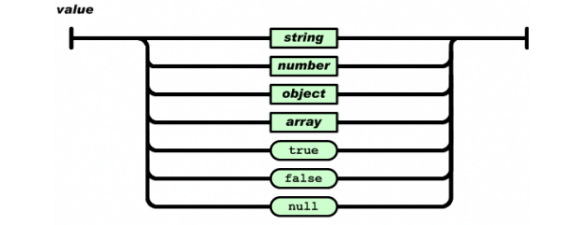
\includegraphics[width=1.0\textwidth]{json2}
	\caption[Cấu trúc của một đối tượng JSON]{Cấu trúc của một đối tượng JSON}
	\label{fig: json2}
\end{figure}

Một giá trị có thể là chuổi, số, đúng sai, hoặc là đối tượng hoặc mảng. Những cấu trúc này có thể được lồng vào nhau.

\textbf{JSON và Webservice}

Việc trao đổi thông tin, truyền tải dữ liệu giữa Webservice và ứng dụng người ta thường dùng XML hay JSON vì sự tiện nghi và cấu trúc dữ liệu nhỏ gọn của nó. JSON là một ngôn ngữ mới với tuổi đời con trẻ nhưng vẫn được ứng dụng nhiều bới những điểm lợi của nó:

• “Con người” có thể đọc được.

• Cú pháp gần với JavaScript nên rất dễ để sử dụng.

• Dữ liệu truyền tải ngắn gọn so với những định dạng dữ liệu như: XML, HTML…

• Việc phân tích (parse) dữ liệu từ dạng chuỗi (nhận từ server) sang dữ liệu có thể sử dụng được (thành Object, Number, Array) dễ dàng.
\begin{figure}[H]
	\centering    
	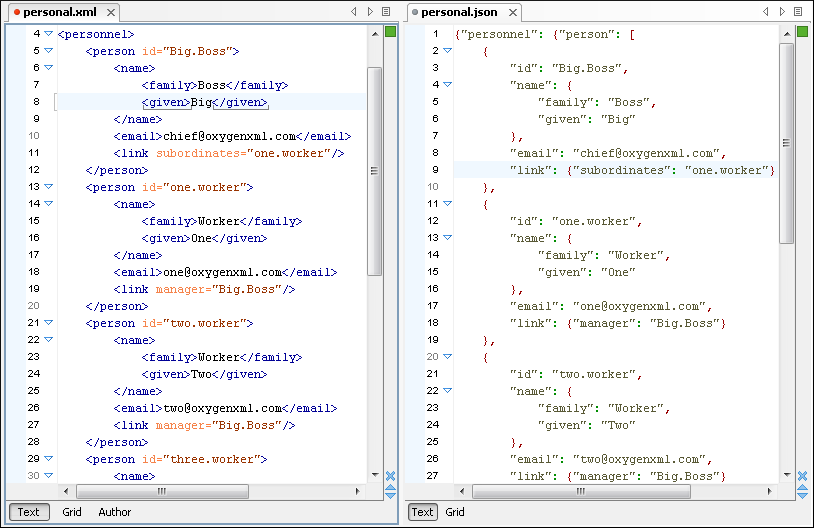
\includegraphics[width=1.0\textwidth]{json3}
	\caption[Cấu trúc mô tả XML-JSON]{Cấu trúc mô tả XML-JSON}
	\label{fig: json3}
\end{figure}
Nhằm mục đích giúp thời gian tương tác giữa người sử dụng với ứng dụng tiến gần đến thời gian thực, thì tốc độ được đặt lên hàng đầu, việc tăng tốc bằng cách “giảm tải” cũng là một giải pháp, chính vì vậy JSON được ưu ái hơn vì cú pháp ngắn gọn, đơn giản, tiết kiệm hơn XML.



\subsection{NodeJs}
%TODO: http://vietjack.com/nodejs/nodejs_la_gi.jsp
NodeJS là một nền tảng Server side được xây dựng dựa trên Javascript Engine (V8 Engine). Node.js được phát triển bởi Ryan Dahl năm 2009. Định nghĩa Nodejs bởi tài liệu chính thức : Node.js là một nền tảng dựa vào Chrome Javascript runtime để xây dựng các ứng dụng nhanh, có độ lớn. 

\begin{figure}[H]
	\centering    
	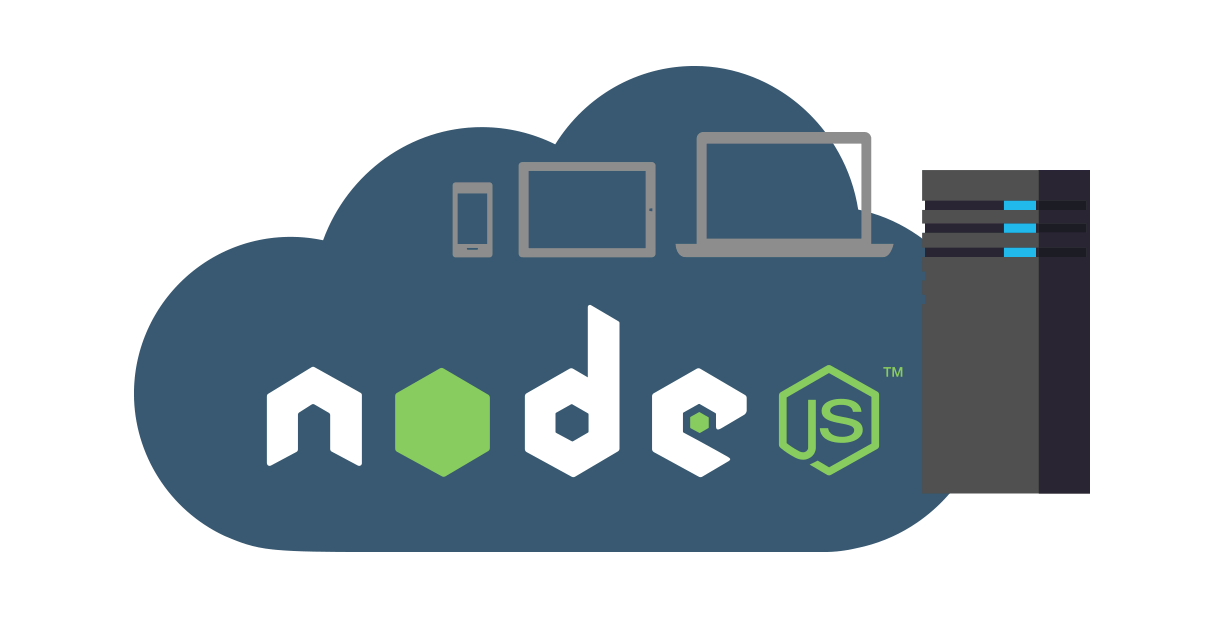
\includegraphics[width=1.0\textwidth]{nodejs0}
	\caption[Nền tảng Nodejs]{Nền tảng Nodejs}
	\label{fig: nodejs0}
\end{figure}

Node.js sử dụng các phần phát sinh các sự kiện (event-driven), mô hình non-blocking I/O để tạo ra các ứng dụng nhẹ và hiệu quả cho các ứng dụng về dữ liệu thời gian thực chạy trên các thiết bị phân tán.

\begin{figure}[H]
	\centering    
	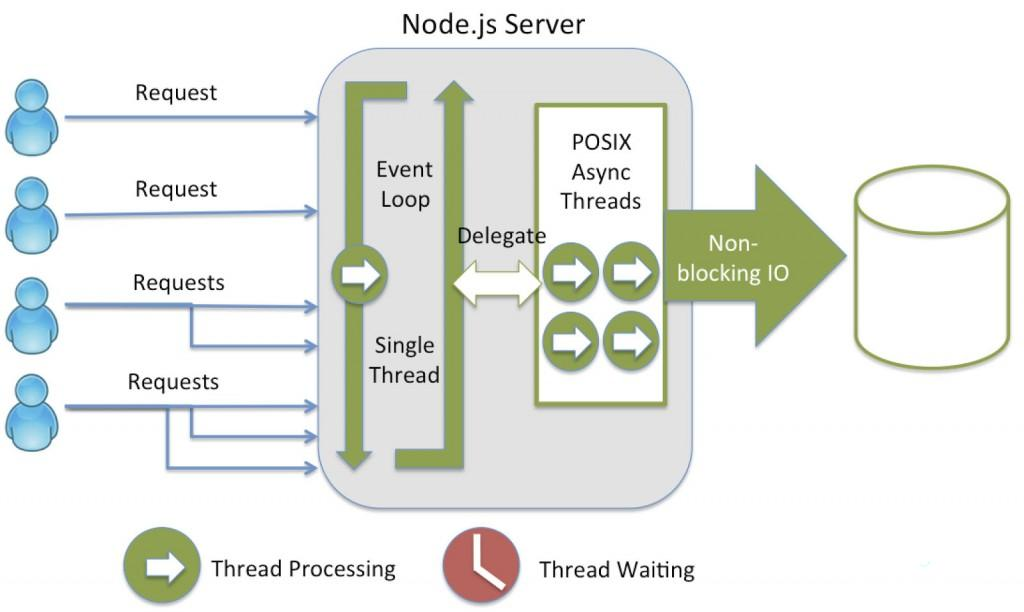
\includegraphics[width=1.0\textwidth]{nodejs1}
	\caption[Mô hình hoạt động Nodejs]{Mô hình hoạt động Nodejs}
	\label{fig: nodejs1}
\end{figure}

\subsection{Javascripts}
%TODO: ref https://vi.wikipedia.org/wiki/JavaScript
JavaScript, theo phiên bản hiện hành, là một ngôn ngữ lập trình kịch bản dựa trên đối tượng được phát triển từ các ý niệm nguyên mẫu. Ngôn ngữ này được dùng rộng rãi cho các trang web, nhưng cũng được dùng để tạo khả năng viết script sử dụng các đối tượng nằm sẵn trong các ứng dụng. Nó vốn được phát triển bởi Brendan Eich tại Hãng truyền thông Netscape với cái tên đầu tiên Mocha, rồi sau đó đổi tên thành LiveScript, và cuối cùng thành JavaScript. Giống Java, JavaScript có cú pháp tương tự C, nhưng nó gần với Self hơn Java. .js là phần mở rộng thường được dùng cho tập tin mã nguồn JavaScript.

%TODO: ref http://freetuts.net/javascript-la-gi-viet-ung-dung-javascript-dau-tien-263.html
Những ứng dụng to lớn của Javascript khiến người ta không thể quên nó được. Hiện nay có rất nhiều libraries, Framework được viêt như:

• AngularJS: Một thư viện dùng để xây dựng ứng dụng Single Page

• NodeJS: Một thư viện được phát triển phía Server dùng để xây dựng ứng dụng realtime

• Sencha Touch: Một Framework  dùng để xây dựng ứng dụng Mobile

• ExtJS: Một Framework dùng xây dựng ứng dụng quản lý (Web Applications)

• jQuery: Một thư viện rất mạnh về hiểu ứng

\subsection{Websocket - Socket.io}
%TODO: http://blog.rikkeisoft.com/seminar-gioi-thieu-ve-websocket-va-node-js/
WebSoket là công nghệ hỗ trợ giao tiếp hai chiều giữa client và server bằng cách sử dụng một TCP socket để tạo một kết nối hiệu quả và ít tốn kém. Mặc dù được thiết kế để chuyên sử dụng cho các ứng dụng web, lập trình viên vẫn có thể đưa chúng vào bất kì loại ứng dụng nào.
\begin{figure}[H]
	\centering    
	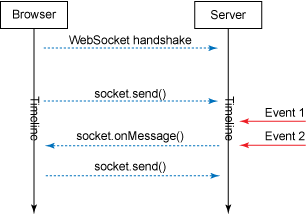
\includegraphics[width=0.5\textwidth]{websk}
	\caption[Mô hình hoạt động Websocket]{Mô hình hoạt động Websocket}
	\label{fig: websk}
\end{figure}

Kết nối được duy trì có thể viết và nhận dữ liệu bằng JavaScript như khi bạn đang sử dụng một TCP socket đơn thuần.

- HTTP: 871 x 10,000 = 8,710,000 bytes = 69,680,000 bits per second (66 Mbps)
- WebSocket: 2 x 10,000 = 20,000 bytes = 160,000 bits per second (0.153 Kbps)


\textbf{Socket.IO}

Socket.IO là một thư viện javascript có mục đích tạo ra các ứng dụng realtime trên trình duyệt cũng như thiết bị di động. Việc sử dụng thư viện này cũng rất đơn giản và giống nhau ở cả server lẫn client. 

\textbf{Tại sao Socket.IO ra đời?}

\begin{itemize}
\item[•]Javascript là ngôn ngữ lập trình hướng sự kiện, mà trong lập trình thời gian thực, cách tiếp cận bằng lập trình sự kiện là cách tiếp cận khôn ngoan nhất.
\item[•]Node.js chạy non-blocking việc hệ thống không phải tạm ngừng để xử lý xong một request sẽ giúp cho server trả lời client gần như ngay tức thì.
\item[•]Lập trình socket yêu cầu bạn phải xây dựng được mô hình lắng nghe – trả lời từ cả 2 bên. Nói khác đi, vai trò của client và server phải tương đương nhau, mà client thì chạy bằng javascript, nên nếu server cũng chạy bằng javascript nữa, thì việc lập trình sẽ dễ dàng và thân thiện hơn.
\end{itemize}

Socket.IO hoạt động dựa trên các events tương tự như Websocket:

• \textbf{connect()}: kết nối với server socket

• \textbf{on(event\_name, listener)}: đăng kí lắng nghe sự kiện từ server trả về

• \textbf{emit(event\_name, data)}: gửi một sự kiện lên server

• \textbf{off(event\_name)}: ngừng lắng nghe một sự kiện nào đó

\subsection{RethinkDB}

\textbf{RethinkDB là gì?}

RethinkDB là một mã nguồn mở, dựa theo cấu trúc cơ sở dữ liệu NoSQL, tổ chức dữ liệu theo kiểu document-oriented database - một thiết kế riêng biệt cho việc lưu trữ document. Các cài đặt có thể là giả lập tương tác trên relational database, object database hay key-value store. Cơ sở dữ liệu được lưu trữ dưới dạng JSON  với các giản đồ động, và được thiết kế giúp hoạt động dễ dàng trong việc cập nhật và truy xuất dữ liệu theo thời gian thực với các ứng dụng. 

\begin{figure}[H]
	\centering    
	
\includegraphics[width=1\textwidth]{rethinkdb}
	\caption[Biểu tượng của RethinkDB]{Biểu tượng của RethinkDB}
	\label{fig: rethinkdb}
\end{figure}

RethinkDB sử dụng ngôn ngữ truy vấn ReQL được phát triển theo hướng đối tượng. Và ngôn ngữ này hỗ trợ cho các thao tác nhập bảng, quản lý nhóm, tích hợp và các hàm chức năng truy vấn cũng như event theo thời gian thực.

\begin{figure}[H]
	\centering    
	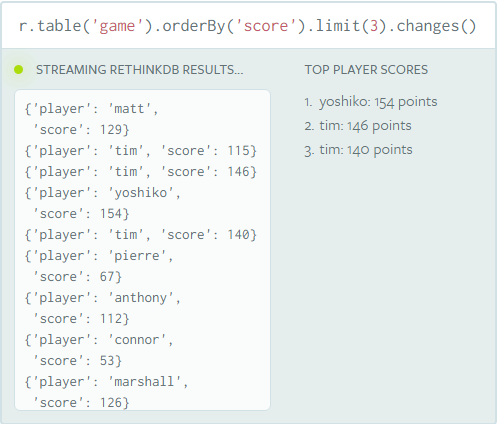
\includegraphics[width=0.9\textwidth]{rethink1}
	\caption[Đoạn code mẫu RethinkDB]{Đoạn code mẫu RethinkDB}
	\label{fig: rethink1}
\end{figure}

Như hình \ref{fig: rethink1} là ví dụ trực quan được demo trực tiếp tại trang chủ https://www.rethinkdb.com, có thể nhận thấy được cách thức khai báo và sử dụng RethinkDB:

• \textbf{r} : là đối tượng RethinkDB chúng ta khai báo trong ứng dụng.

• \textbf{table()} : là bảng giá trị đang truy vấn.

• \textbf{orderBy()} : hàm sắp xếp dữ liệu theo trường giá trị được khai báo.

• \textbf{limit()} : chọn ra những giá trị trong phạm vi được khai báo trong hàm.

• \textbf{changes()} : đây chính là đặc điểm khiến RethinkDB khác biệt so với các hệ quản lý dữ liệu khác. RethinkDB sẽ gọi hàm thực thi khi vùng giá trị truy vấn có thay dổi giá trị theo thời gian thật. không hoạt động theo cơ chế polling thường thấy ở các kiểu truy vấn dữ liệu khác.

%TODO: tham khảo tại https://vi.wikipedia.org/wiki/NoSQL
\subsection{Raspberry}

Raspbian là hệ điều hành mở và miễn phí được phát triển tối ưu hóa dựa trên nền Debian dành riêng cho thiết bị phần cứng Raspberry Pi. Hệ điều hành này bao gồm nhóm các chức năng và ứng dụng giúp Raspberry hoạt động. Hơn nữa, Raspbian cung cấp nhiều hơn là hệ điều hành thuần: hỗ trợ tới hơn 35,000 gói mở rộng và dễ dàng cài đặt trên Raspberry Pi. Raspbian ổn định và hiệu suất cao được hoàn thiện vào tháng 6 năm 2012. Tuy nhiên Raspbian vẫn đang được phát triển tới ngày nay và ngày càng cải thiện hiệu suất cũng như hỗ trợ các gói chức năng nhiều nhất có thể.
\begin{figure}[H]
	\centering    
	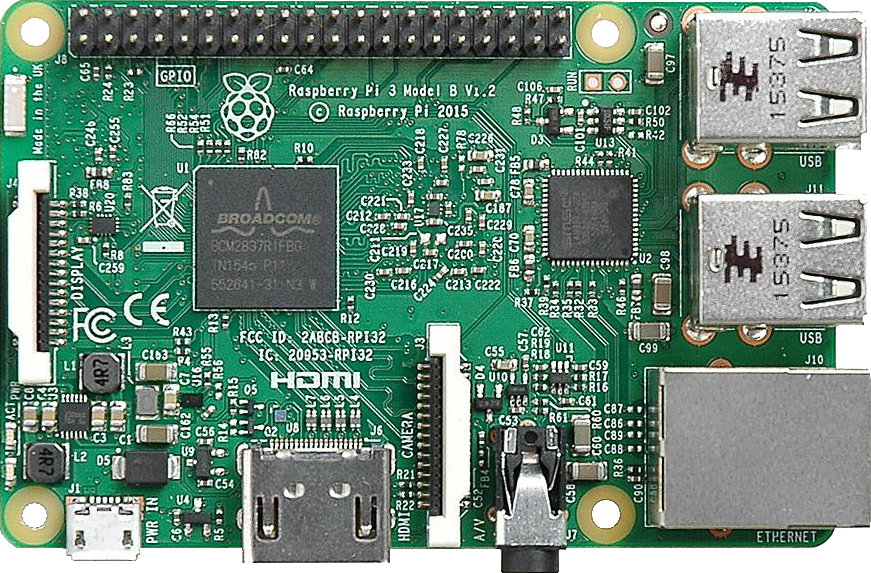
\includegraphics[width=0.9\textwidth]{rasp}
	\caption[Thiết bị Raspberry Pi]{Thiết bị Raspberry Pi}
	\label{fig: rasp}
\end{figure}

Vì sao lựa chọn Raspberry:

• Là một máy tính độc lập chạy trên nền tảng Linux, điều này làm cho việc chạy các ứng dụng Nodejs hay RethinkDB hoạt động được trên Raspberry Pi.

• Hiệu suất đáp ứng nhu cầu làm server của đề tài yêu cầu với mức độ tiêu thụ năng lượng cực kì ít.

\subsection{Framework Ionic}
\subsection*{Giới thiệu về Ionic framework}
Ionic là một framework được sử dụng để phát triển các ứng dụng di động dựa trên nền tảng công nghệ web HTML5 để tạo ra các ứng dụng lai hóa [ hybrid apps ] chạy trên các thiết bị di động khác nhau. Ứng dụng lai hóa ở đây được hiểu cơ bản là các ứng dụng chạy trên nền các trình duyệt được nhúng vào trong một ứng dụng được cài đặt và có thể giao tiếp, truy cập, điều khiển sử dụng các thiết bị phần cứng và hệ điều hành mobile.

Hãy tưởng tượng Ionic như là một khung phát triển giao diện người dùng để xử lý tất cả các tương tác giao diện người dùng làm cho ứng dụng trở nên thuyết phục và dễ dàng sử dụng. Kiểu như “Bootstrap for Native”, tức là như các ứng dụng Native nhưng có sự hỗ bởi một loạt các thành phần giao diện, động và thiết kế đẹp.

\begin{center}
\begin{figure}[htp]
\centering    
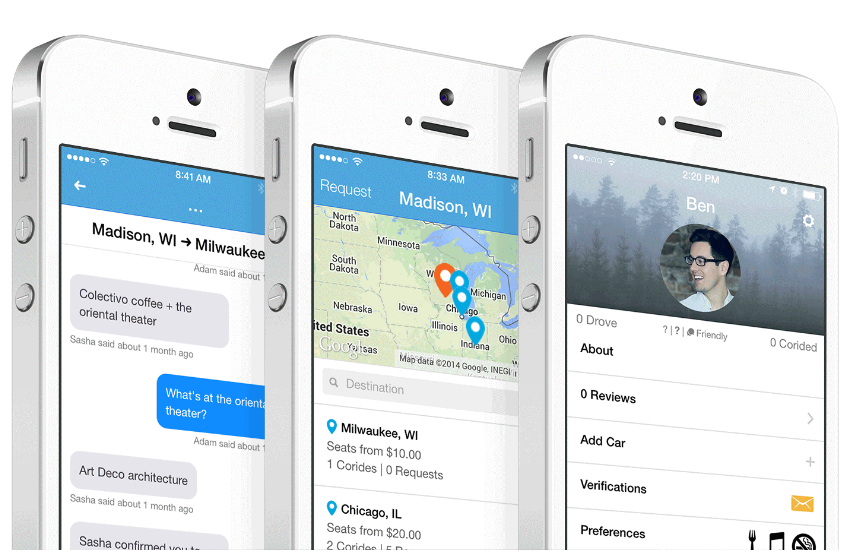
\includegraphics[width=0.7\textwidth]{ionic}
\caption[Một số giao diện của Ionic ]{Một số giao diện của Ionic}
\label{fig:ionic}
\end{figure}
\end{center}


Bản chất Ionic là một khung phát triển HTML5, nó cần một vỏ bọc native như Cordova hay PhoneGap để có thể khởi động như một ứng dụng native. Ionic được hỗ trợ mạnh mẽ bởi Cordova. Việc cài đặt và khởi tạo một dự án Ionic rất dễ dàng thông qua giao diện dòng lệnh dựa trên Node.js


\subsection*{Ưu điểm và nhược điểm của Ionic}

\subsubsection*{Ưu điểm }
\begin{itemize}
\item[•] Dễ học, thời gian phát triển nhanh, có thể sử dụng các kỹ năng từ lập trình web.
\item[•] Đa nền tảng.
\item[•] Khả năng truy cập đến các tính năng của thiết bị và hệ điều hành như bluetooth, camera,..
\item[•] Dễ dàng thiết kế giao diện cho các thiết bị có kích cỡ khác nhau
\item[•] Việc sử dụng AngularJS làm core giúp phần xử lý UI linh động hơn so với javasript hay thư viện Jquery.
\item[•] Việc sử dụng AngularJS làm core cũng mang lại lợi thế lớn so với các framework cho ứng dụng hybrid khác.
\item[•] Ionic cung cấp đầy đủ các thành phần trong giao diện người dùng như Pull-to-Refresh, Infinite-loader, tabs, …

\end{itemize}


\subsubsection*{Nhược điểm }


\begin{itemize}
\item[•] Vẫn còn trong giai đoạn phát triển.
\item[•] Hiệu năng vẫn chưa cao và ổn định.
\item[•] Cộng đồng phát triển ứng dụng vẫn còn chưa đông.
\end{itemize}

\subsection{Framework AngularJS}



Angular là một bộ Javascript Framework rất mạnh và thường được sử dụng để xây dựng project Single Page Application (SPA). Nó hoạt động dựa trên các thuộc tính mở rộng HTML (các atributes theo quy tắc của Angular). Đây là một Framework mã nguồn mở hoàn toàn miễn phí và được hàng ngàn các lập trình viên trên thế giới ưa chuộng và sử dụng.


\begin{center}
\begin{figure}[htp]
\centering    

\includegraphics[width=0.7\textwidth]{angularjs}
\caption[Angular JS kết hợp với ionic ]{Angular JS kết hợp với ionic}
\label{fig:angularjs}
\end{figure}
\end{center}

Ionic sử dụng AngularJS để cung cấp các cấu trúc ứng dụng, trong khi bản thân Ionic tập trung chính vào giao diện người dùng. Nói cách khác, chúng ta thấy được sự phối hợp ăn ý giữa sức mạnh của AngularJS và vẻ đẹp của Ionic UI.

Ionic cung cấp một tập các Angular directives (nghĩa là các phần tử HTML tùy biến) để làm các thành phần của nó, tạo ra sự dễ dàng để sử dụng các tiện ích gọn để viết mã HTML. Ngoài các directives, Ionic còn sử dụng và thêm vào các thành phần khác như: Angular touch recognizers, view animation logic, HTML sanitation, và asynchronous communication.

Việc xây dựng ứng dụng dựa trên AngularJS đòi hỏi mã nguồn phải có khả năng mở rộng cao để bổ sung các tính năng mới. Tuy nhiên với Ionic, người ta có thể tái sử dụng các chức năng trong ứng dụng trên các nền tảng khác nhau đồng thời vẫn có thể tùy chỉnh giao diện người dùng cho mỗi nền tảng riêng biệt. Các thành phần trong Ionic như danh sách, slide,.. chính là các directive(các thuộc tính của thẻ HTML dùng trong Angular) của AngularJS. Đó là lí do khiến cho Ionic và AngularJS kết hợp rất tốt với nhau.

Mặc dù, Ionic có thành phần giao diện sử dụng Angular, nhưng developers vẫn có thể sử dụng và hỗ trợ các framework khác như Knockout hay EmberJS.



\subsection{Framework Cordova}

\begin{center}
\begin{figure}[htp]
\centering    

\includegraphics[width=0.7\textwidth]{cordova}
\caption[Apache Cordova ]{Apache Cordova}
\label{fig:cordova}
\end{figure}
\end{center}

Apache Cordova là một bộ khung để xây dựng ứng dụng di động sử dụng HTML, CSS và Javascript. Apache Cordova bao gồm một tập hợp các API thiết bị cho phép người lập trình di động truy cập, sử dụng các chức năng native của thiết bị như là camera hay cảm biến gia tốc bằng Javascript. Kết hợp với một bộ khung phát triển giao diện như jQuery Mobile or Dojo Mobile hoặc Ionic, cho phép ứng dụng di động có thể được phát triển chỉ dựa trên HTML, CSS và Javascript.

Khi sử dụng Cordova API, một ứng dụng có thể được xây dựng mà không phải sử dụng bất kỳ một đoạn mã native code nào. Thay vào đó, công nghệ web sẽ được sử dụng, và chúng sẽ được tổ chức trên chính ứng dụng đấy chứ không cần thông qua một server nào.

Cordova cung cấp một tập hợp các thư viện Javascript đã được chuẩn hóa để có thể sử dụng. Cordova hiện có thể sử dụng cho các nền tảng như iOS, Android, Blackberry, Windows Phone, Palm WebOS, Bada và Symbian.

